\documentclass[10pt,letterpaper]{article}

\usepackage[utf8]{inputenc}
\usepackage{cvpr}
\usepackage{times}
\usepackage{epsfig}
\usepackage{graphicx}
\usepackage{amsmath,amsfonts,amssymb,amsthm}
\usepackage{xcolor}
\usepackage{caption}
\usepackage{subcaption}
\usepackage{xspace}
\usepackage{array}
\usepackage{cite}
\usepackage[pagebackref=true,breaklinks=true,colorlinks,bookmarks=false]{hyperref}
\usepackage{tabularx}
\usepackage{multirow}

\newcommand{\Perp}{\perp\!\!\! \perp}
\newcommand{\bK}{\mathbf{K}}
\newcommand{\bX}{\mathbf{X}}
\newcommand{\bY}{\mathbf{Y}}
\newcommand{\bk}{\mathbf{k}}
\newcommand{\bx}{\mathbf{x}}
\newcommand{\by}{\mathbf{y}}
\newcommand{\bhy}{\hat{\mathbf{y}}}
\newcommand{\bty}{\tilde{\mathbf{y}}}
\newcommand{\bG}{\mathbf{G}}
\newcommand{\bI}{\mathbf{I}}
\newcommand{\bg}{\mathbf{g}}
\newcommand{\bS}{\mathbf{S}}
\newcommand{\bs}{\mathbf{s}}
\newcommand{\bM}{\mathbf{M}}
\newcommand{\bw}{\mathbf{w}}
\newcommand{\eye}{\mathbf{I}}
\newcommand{\bU}{\mathbf{U}}
\newcommand{\bV}{\mathbf{V}}
\newcommand{\bW}{\mathbf{W}}
\newcommand{\bn}{\mathbf{n}}
\newcommand{\bv}{\mathbf{v}}
\newcommand{\bq}{\mathbf{q}}
\newcommand{\bR}{\mathbf{R}}
\newcommand{\bi}{\mathbf{i}}
\newcommand{\bj}{\mathbf{j}}
\newcommand{\bp}{\mathbf{p}}
\newcommand{\bt}{\mathbf{t}}
\newcommand{\bJ}{\mathbf{J}}
\newcommand{\bu}{\mathbf{u}}
\newcommand{\bB}{\mathbf{B}}
\newcommand{\bD}{\mathbf{D}}
\newcommand{\bz}{\mathbf{z}}
\newcommand{\bP}{\mathbf{P}}
\newcommand{\bC}{\mathbf{C}}
\newcommand{\bA}{\mathbf{A}}
\newcommand{\bZ}{\mathbf{Z}}
\newcommand{\bff}{\mathbf{f}}
\newcommand{\bF}{\mathbf{F}}
\newcommand{\bo}{\mathbf{o}}
\newcommand{\bO}{\mathbf{O}}
\newcommand{\bc}{\mathbf{c}}
\newcommand{\bm}{\mathbf{m}}
\newcommand{\bT}{\mathbf{T}}
\newcommand{\bQ}{\mathbf{Q}}
\newcommand{\bL}{\mathbf{L}}
\newcommand{\bl}{\mathbf{l}}
\newcommand{\ba}{\mathbf{a}}
\newcommand{\bE}{\mathbf{E}}
\newcommand{\bH}{\mathbf{H}}
\newcommand{\bd}{\mathbf{d}}
\newcommand{\br}{\mathbf{r}}
\newcommand{\be}{\mathbf{e}}
\newcommand{\bb}{\mathbf{b}}
\newcommand{\bh}{\mathbf{h}}
\newcommand{\bhh}{\hat{\mathbf{h}}}
\newcommand{\btheta}{\boldsymbol{\theta}}
\newcommand{\bTheta}{\boldsymbol{\Theta}}
\newcommand{\bpi}{\boldsymbol{\pi}}
\newcommand{\bphi}{\boldsymbol{\phi}}
\newcommand{\bPhi}{\boldsymbol{\Phi}}
\newcommand{\bmu}{\boldsymbol{\mu}}
\newcommand{\bSigma}{\boldsymbol{\Sigma}}
\newcommand{\bGamma}{\boldsymbol{\Gamma}}
\newcommand{\bbeta}{\boldsymbol{\beta}}
\newcommand{\bomega}{\boldsymbol{\omega}}
\newcommand{\blambda}{\boldsymbol{\lambda}}
\newcommand{\bLambda}{\boldsymbol{\Lambda}}
\newcommand{\bkappa}{\boldsymbol{\kappa}}
\newcommand{\btau}{\boldsymbol{\tau}}
\newcommand{\balpha}{\boldsymbol{\alpha}}
\newcommand{\nR}{\mathbb{R}}
\newcommand{\nN}{\mathbb{N}}
\newcommand{\nL}{\mathbb{L}}
\newcommand{\nF}{\mathbb{F}}
\newcommand{\cN}{\mathcal{N}}
\newcommand{\cM}{\mathcal{M}}
\newcommand{\cR}{\mathcal{R}}
\newcommand{\cB}{\mathcal{B}}
\newcommand{\cL}{\mathcal{L}}
\newcommand{\cH}{\mathcal{H}}
\newcommand{\cS}{\mathcal{S}}
\newcommand{\cT}{\mathcal{T}}
\newcommand{\cO}{\mathcal{O}}
\newcommand{\cC}{\mathcal{C}}
\newcommand{\cP}{\mathcal{P}}
\newcommand{\cE}{\mathcal{E}}
\newcommand{\cF}{\mathcal{F}}
\newcommand{\cK}{\mathcal{K}}
\newcommand{\cY}{\mathcal{Y}}
\newcommand{\cX}{\mathcal{X}}
\def\bgamma{\boldsymbol\gamma}

\newcommand{\specialcell}[2][c]{%
  \begin{tabular}[#1]{@{}c@{}}#2\end{tabular}}

\newcommand{\figref}[1]{\Fig~\ref{#1}}
\newcommand{\secref}[1]{Section~\ref{#1}}
%\renewcommand{\algref}[1]{Algorithm~\ref{#1}}
\newcommand{\eqnref}[1]{Eq.~\eqref{#1}}
\newcommand{\tabref}[1]{Table~\ref{#1}}

\newcommand{\rulesep}{\unskip\ \vrule\ }

\DeclareMathOperator*{\argmax}{argmax~}
\DeclareMathOperator*{\argmin}{argmin~}
\DeclareMathOperator{\sign}{sign}

\renewcommand{\b}{\ensuremath{\mathbf}}

\def\mc{\mathcal}
\def\mb{\mathbf}

\newcommand{\T}{^{\raisemath{-1pt}{\mathsf{T}}}}

\makeatletter
\DeclareRobustCommand\onedot{\futurelet\@let@token\@onedot}
\def\@onedot{\ifx\@let@token.\else.\null\fi\xspace}
\def\eg{e.g\onedot} \def\Eg{E.g\onedot}
\def\ie{i.e\onedot} \def\Ie{I.e\onedot}
\def\cf{cf\onedot} \def\Cf{Cf\onedot}
\def\etc{etc\onedot} \def\vs{vs\onedot}
\def\wrt{wrt\onedot}
\def\dof{d.o.f\onedot}
\def\etal{et~al\onedot} \def\iid{i.i.d\onedot}
\def\Fig{Fig\onedot} \def\Eqn{Eqn\onedot} \def\Sec{Sec\onedot} \def\Alg{Alg\onedot}
\makeatother

% nice url font and color
\renewcommand\UrlFont{\color{blue}\rmfamily}

% rotation
\newcommand*\rot{\rotatebox{90}}
\newcommand{\boldparagraph}[1]{\vspace{0.2cm}\noindent{\bf #1:} }

% comments
\definecolor{darkgreen}{rgb}{0,0.7,0}
\newcommand{\ag}[1]{ \noindent {\color{red} {\bf Andreas:} {#1}} }
\newcommand{\red}[1]{\noindent{\color{red}{#1}}}
%\newcommand{\green}[1]{\noindent{\color{darkgreen}{#1}}}
\newcommand{\green}[1]{#1}

% https://tex.stackexchange.com/questions/128496/elegant-fractions-in-one-line
\newcommand{\uk}{\ensuremath{\bot}}

% methods
\newcommand{\AML}{AML\xspace}
\newcommand{\ML}{ML\xspace}
\newcommand{\Sup}{Sup\xspace}
\newcommand{\Mean}{Mean\xspace}
\newcommand{\VAE}{VAE\xspace}
\newcommand{\VAEs}{VAEs\xspace}
\newcommand{\clean}{SN-clean\xspace}
\newcommand{\noisy}{SN-noisy\xspace}
\newcommand{\Abs}{Ham\xspace}
\newcommand{\Acc}{Acc\xspace}
\newcommand{\Compl}{Comp\xspace}
\newcommand{\PPCA}{PPCA\xspace}
\newcommand{\PCA}{PCA\xspace}

% colors
\definecolor{rred}{rgb}{0.65,0.23,0.25}
\definecolor{rbeige}{rgb}{0.66,0.45,0.23 }
\definecolor{rgreen}{rgb}{0.22,0.54,0.19}

\cvprfinalcopy
\def\cvprPaperID{1708}
\def\httilde{\mbox{\tt\raisebox{-.5ex}{\symbol{126}}}}
%\ifcvprfinal\pagestyle{empty}\fi

\RequirePackage{snapshot}
\begin{document}
	
\title{Supplementary Material for\\\green{Learning 3D Shape Completion from Laser Scan Data with Weak Supervision}}
\author{David Stutz$^{1,2}$ \qquad Andreas Geiger$^{1,3}$\\
	$^1$Autonomous Vision Group, MPI for Intelligent Systems and University of Tübingen\\
	$^2$Computer Vision and Multimodal Computing, Max-Planck Institute for Informatics, Saarbr\"{u}cken\\
	$^3$Computer Vision and Geometry Group, ETH Z\"{u}rich\\
	{\tt\small david.stutz@mpi-inf.mpg.de,andreas.geiger@tue.mpg.de}	
}

\clearpage\maketitle
%\ifcvprfinal\thispagestyle{empty}\fi

\section{Overview}
\label{sec:appendix-overview}

This document provides additional details regarding the used datasets and further experimental results complementary to the main paper. In Section \ref{sec:appendix-data}, we discuss technical details regarding the introduced, synthetic datasets derived from ShapeNet \cite{Chang2015ARXIV}, referred to as \clean and \noisy, \green{the synthetic dataset derived from ModelNet \cite{Wu2015CVPR},} as well as the dataset extracted from KITTI \cite{Geiger2012CVPR}. \green{Then, in Section \ref{sec:appendix-architecture}, we provide additional details concerning architecture followed by a discussion of the training procedure in Section \ref{sec:appendix-training}.} In Section \ref{sec:appendix-evaluation}, we discuss our implementation of the mesh-to-mesh distance used for evaluation. Subsequently, in Section \ref{sec:appendix-baselines} we discuss the evaluation of the approach by Engelmann \etal \cite{Engelmann2016GCPR} in more detail and, finally, present additional experiments in Section~\ref{sec:appendix-experiments}.

\section{Data}
\label{sec:appendix-data}

\boldparagraph{ShapeNet}
%
For generating \clean and \noisy, we took a subset of the car models provided by ShapeNet, simplified them, generated several random variants of each model and scaled them to allow signed distance function (SDF) computation. Specifically, we obtained $3253$ car models from ShapeNet \cite{Chang2015ARXIV} after manually discarding $262$ of the available $3515$ car models. The discarded models could not be oriented or scaled automatically and mostly correspond to large, elongated or exotic cars -- see Figure \ref{fig:appendix-experiments-shapenet} (left) for examples. We subsequently simplified the models using the semi-convex hull algorithm described in \cite{Guney2015CVPR} as illustrated in Figure \ref{fig:appendix-experiments-shapenet} (middle). This was necessary for two reasons: to reduce the complexity of the models (\ie, reduce the number of faces from up to $\sim 1700k$ to exactly $1k$); and to obtain watertight meshes. While we would expect the majority of the car models to be approximately watertight, this is not always the case -- often, we found cars without windows or with open doors. We scaled the simplified models to $[-0.5, 0.5]^3$ (centered at the origin; padded by $0.1$ on all sides) in order to randomly scale (by factors in $(0.9, 1.05)$), randomly rotate (by $-2.5$ to $2.5$, $-5$ to $5$ and $-2.5$ to $2.5$ degrees around the x, y and z axes, respectively), randomly translate (by $[-0.1,0.1] \times [-0.05,0.05] \times [-0.05,0.05]$) and obtain $10$ variants per model ($6$ for the validation set). We note that, in our case, x,y and z axes correspond to length, height and breadth of the cars; or x = right, y = up and z = forward. The models are then translated to $(0.5, 0.5, 0.5)$ and scaled by $W$ to fit the voxel grid $H \times W \times D$ (for the voxel grid, x and y axes are flipped).

Based on the pre-processed models, we compute SDFs, occupancy grids and derive observations. To this end, considering watertight meshes, we make the following observation: a ray from the origin (outside of the mesh) to a voxel's center (\ie, $(w + 0.5, h + 0.5, d + 0.5)$ for $0\leq w<W$, $0\leq h<H$ and $0\leq d<D$), intersects the mesh surface an odd number of times if and only if the voxel's center lies inside of the mesh. Thus, for each voxel center, we compute the distance to the surface (using point-to-triangle distance\footnote{We use the code provided by Christopher Batty at \url{https://github.com/christopherbatty/SDFGen}.}) and assign negative sign if the voxel's center is found to be inside the mesh (using ray-triangle intersections \cite{Moller1997JGT}\footnote{We use the code provided at \url{http://fileadmin.cs.lth.se/cs/personal/tomas_akenine-moller/code/}.}). The corresponding occupancy grids are derived by thresholding. To derive observations, we use the OpenGL renderer of \cite{Guney2015CVPR} and subsequently back-project the pixels to 3D using the known camera calibration matrix; this process is illustrated in Figure \ref{fig:appendix-experiments-shapenet} (right). To obtain observations from different viewpoints, we randomly rotate the camera around the cars ($360$ degrees). \green{For \noisy, we additionally add exponentially-distributed error (with rate parameter $70$) to the depth values or set them to the maximum depth with probability $0.075$.} The observed points can directly be voxelized; to compute free space, we perform ray tracing (from the camera center to the observed points) by computing ray-voxel intersections \cite{Williams2005SIGGRAPH}\footnote{We use the code provided at \url{http://www.cs.utah.edu/~awilliam/box/}.} along the rays. We note that we do not perform ray tracing for background points as we do not have any notion of background on KITTI.

\begin{figure*}
    \centering
    \begin{subfigure}[t]{0.31\textwidth}
        \vspace{0px}
        \centering
        \begin{subfigure}[t]{0.475\textwidth}
            \vspace{0px}
            \centering
            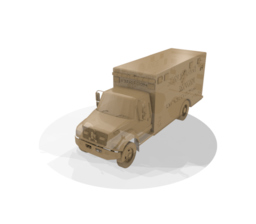
\includegraphics[width=2.5cm,trim={0.25cm 0.5cm 1.5cm 1.5cm},clip]{gfx/appendix_experiments_shapenet/meshes/00014}
        \end{subfigure}
        \begin{subfigure}[t]{0.475\textwidth}
            \vspace{0px}
            \centering
            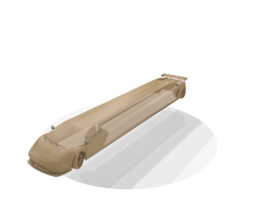
\includegraphics[width=2.5cm,trim={0.25cm 0.5cm 1.5cm 1.5cm},clip]{gfx/appendix_experiments_shapenet/meshes/00007}
        \end{subfigure}\\
        \begin{subfigure}[t]{0.475\textwidth}
            \vspace{0px}
            \centering
            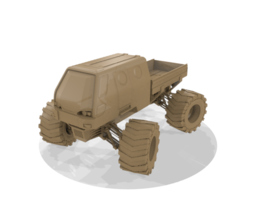
\includegraphics[width=2.5cm,trim={0.25cm 0.5cm 1.5cm 1.5cm},clip]{gfx/appendix_experiments_shapenet/meshes/00017}
        \end{subfigure}
        \begin{subfigure}[t]{0.475\textwidth}
            \vspace{0px}
            \centering
            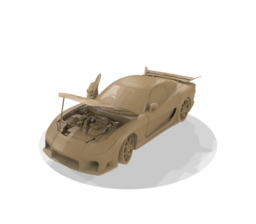
\includegraphics[width=2.5cm,trim={0.25cm 0.5cm 1.5cm 1.5cm},clip]{gfx/appendix_experiments_shapenet/meshes/00013}
        \end{subfigure}
    \end{subfigure} 
    {\color{black!25}\vrule width 0.5px}
    \begin{subfigure}[t]{0.31\textwidth}
        \vspace{0px}
        \centering
        \begin{subfigure}[t]{0.475\textwidth}
            \vspace{0px}
            \centering
            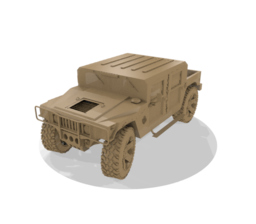
\includegraphics[width=2.5cm,trim={0.25cm 0.5cm 1.5cm 1.5cm},clip]{gfx/appendix_experiments_shapenet/meshes/00000}
        \end{subfigure}
        \begin{subfigure}[t]{0.475\textwidth}
            \vspace{0px}
            \centering
            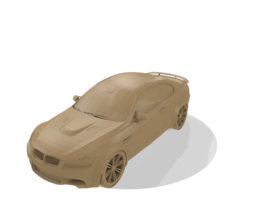
\includegraphics[width=2.5cm,trim={0.25cm 0.5cm 1.5cm 1.5cm},clip]{gfx/appendix_experiments_shapenet/meshes/00002}
        \end{subfigure}\\
        \begin{subfigure}[t]{0.475\textwidth}
            \vspace{0px}
            \centering
            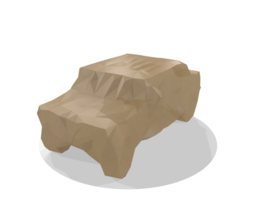
\includegraphics[width=2.5cm,trim={0.25cm 0.5cm 1.5cm 1.5cm},clip]{gfx/appendix_experiments_shapenet/meshes/00001}
        \end{subfigure}
        \begin{subfigure}[t]{0.475\textwidth}
            \vspace{0px}
            \centering
            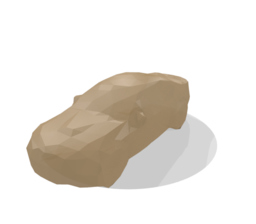
\includegraphics[width=2.5cm,trim={0.25cm 0.5cm 1.5cm 1.5cm},clip]{gfx/appendix_experiments_shapenet/meshes/00003}
        \end{subfigure}
    \end{subfigure}
    {\color{black!25}\vrule width 0.5px}
    \begin{subfigure}[t]{0.31\textwidth}
        \vspace{0px}
        \centering
        \begin{subfigure}[t]{0.475\textwidth}
            \vspace{0px}
            \centering
            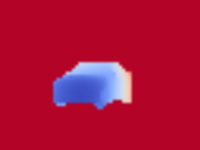
\includegraphics[width=2.5cm]{gfx/appendix_experiments_shapenet/depths/18}
        \end{subfigure}
        \begin{subfigure}[t]{0.475\textwidth}
            \vspace{0px}
            \centering
            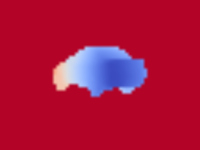
\includegraphics[width=2.5cm]{gfx/appendix_experiments_shapenet/depths/54}
        \end{subfigure}\\[0.15cm]
        \begin{subfigure}[t]{0.475\textwidth}
            \vspace{0px}
            \centering
            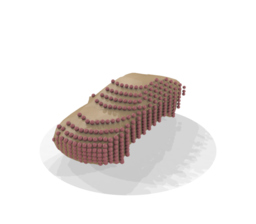
\includegraphics[width=2.5cm,trim={0.25cm 0.5cm 1.5cm 1.5cm},clip]{gfx/experiments_data/clean*/simplified/00001}
        \end{subfigure}
        \begin{subfigure}[t]{0.475\textwidth}
            \vspace{0px}
            \centering
            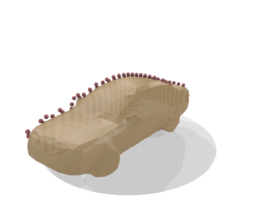
\includegraphics[width=2.5cm,trim={0.25cm 0.5cm 1.5cm 1.5cm},clip]{gfx/experiments_data/clean*/simplified/00009}
        \end{subfigure}
    \end{subfigure}
    \caption{{\bf Left: Examples of Discarded ShapeNet Models.} We manually discarded 262 of ShapeNet's \cite{Chang2015ARXIV} car models by inspecting top-views of the corresponding meshes. Most of the discarded models represent large, elongated or exotic cars such as trucks, limousines or monster trucks. Other models also include opened doors or other unwanted settings. {\bf Middle: Simplification Examples.} The used simplification algorithm \cite{Guney2015CVPR} reduces all models to exactly $1k$ faces; for some models this results in crude approximations, for others, only minor details are lost. We show the original models (top) and the corresponding simplified models (bottom). {\bf Right: Rendering Examples.} Illustration of our rendering process for \clean where a model is rendered into a depth image from a random viewpoint around the car. We show the rendered depth image (top; {\color{red}red} is background, {\color{blue}blue} is closer) and the corresponding model (bottom; {\color{rbeige}beige}) including observations (bottom; {\color{rred}red}).}
    \label{fig:appendix-experiments-shapenet}
\end{figure*}

\boldparagraph{KITTI}
%
On KITTI, we obtained observations by extracting the ground truth 3D bounding boxes of KITTI's 3D object detection benchmark. As the bounding boxes are tightly fitted, we first padded them by factor $0.25$ on all sides. Then, if $l$ denotes the length of a particular bounding box / car after padding (\ie, its size along the x axis), we scaled the bounding box by factor $\frac{W}{l}$; afterwards, the observed points can directly be voxelized into the voxel grid of size $H \times W \times D$. Based on the average bounding box, we determined $H \times W \times D = 24 \times 54 \times 24$. We also note that the 3D bounding box annotations are in camera coordinates, while the point clouds are in Velodyne coordinates -- this can be accounted for using the Velodyne-to-camera transformation as detailed in \cite{Geiger2013IJRR}. To not take points from the street or nearby walls, vegetation or objects into account, we only considered those points lying within the original (\ie, not padded) bounding box. Finally, free space is computed using ray tracing as described above.

For evaluation, we generated ground truth point clouds by accumulating points from multiple frames. In particular, for each ground truth bounding box, we considered the corresponding tracklet in KITTI's raw annotations. Again, we note that the 3D bounding boxes of the 3D object detection benchmark are in camera coordinates, while the 3D bounding boxes from the raw annotations are in Velodyne coordinates which we accounted for as described above. Overall, we considered $10$ future and $10$ past frames in $0.5s$ intervals (\ie, each 5th frame) going a total of $50$ frames / $5s$ into the future and the past, respectively. We found that considering more frames (or smaller intervals) does not contribute to more complete observations of the cars. Finally, the ground truth points are scaled and voxelized as described above. On average, we used $6$ frames per sample to obtain $597$ points (compared to, on average, $128$ points in the observations) on the validation set.

\begin{table}
    \centering
    \vspace*{-0.25cm}
    \begin{subfigure}[t]{0.49\textwidth}
    	\vspace{0px}
        % clean
        % -----
        % [Data] set: validation.json
        % [Data] N: 1950
        % [Data] pixels: 31104
        % [Data] points: 411.713333333
        % [Data] occupied: 3525
        % [Data] observed points: 331.593333333
        % [Data] observed space: 2190.67692308
        % [Data] observed total: 2522.27025641
        % [Data] observed invalid: 24.0307692308
        % [Data] set: training_prior.json
        % [Data] N: 14640
        % [Data] pixels: 31104
        % [Data] points: 407.848838798
        % [Data] occupied: 3522
        % [Data] observed points: 329.771857923
        % [Data] observed space: 2193.04344262
        % [Data] observed total: 2522.8135929
        % [Data] observed invalid: 24.9206967213
        % [Data] set: training_inference.json
        % [Data] N: 14640
        % [Data] pixels: 31104
        % [Data] points: 410.855874317
        % [Data] occupied: 3574
        % [Data] observed points: 331.223702186
        % [Data] observed space: 2200.80642077
        % [Data] observed total: 2532.03224044
        % [Data] observed invalid: 27.4879098361
        % noisy
        % -----
        % [Data] set: training_inference.json
        % [Data] N: 14640
        % [Data] pixels: 31104
        % [Data] points: 106.733538251
        % [Data] occupied: 3574
        % [Data] observed points: 100.450819672
        % [Data] observed space: 1507.3431694
        % [Data] observed total: 1607.79535519
        % [Data] observed invalid: 143.542076503
        % [Data] set: validation.json
        % [Data] N: 1950
        % [Data] pixels: 31104
        % [Data] points: 106.267692308
        % [Data] occupied: 3525
        % [Data] observed points: 100.188205128
        % [Data] observed space: 1483.26205128
        % [Data] observed total: 1583.45025641
        % [Data] observed invalid: 136.838461538
        % [Data] set: training_prior.json
        % [Data] N: 14640
        % [Data] pixels: 31104
        % [Data] points: 105.880737705
        % [Data] occupied: 3522
        % [Data] observed points: 99.7855874317
        % [Data] observed space: 1499.75751366
        % [Data] observed total: 1599.54357923
        % [Data] observed invalid: 142.554098361
        
        {\small
        \begin{tabularx}{1\textwidth}{|X|c|c|}
            \hline
            \clean and \noisy & \clean & \noisy\\
            \hline
            \#Models (Prior / Inference / Val) & \multicolumn{2}{c|}{325 / 1464 / 1464}\\ % = 3253
            \#Samples (Prior / Inference / Val) & \multicolumn{2}{c|}{1950 / 14640 / 1464}\\
            \hline
            Avg. \#Points & 411 & 106\\
            \% Observed / Free Space Voxels & 1.06 / 7.04 & 0.32 / 4.8\\
            %\% Free Space Voxels & 7.04 & 4.8\\
            \% Invalid Free Space Voxels & 0.078 & 0.44\\
            \hline
        \end{tabularx}
        }
        % training
        % --------
        % [Data] N: 7140
        % [Data] pixels: 31104
        % [Data] points: 135.218907563
        % [Data] observed frames: 7
        % [Data] observed points: 135
        % [Data] observed points (combined GT): 855
        % [Data] observed points voxels: 95.9831932773
        % [Data] observed points voxels (combined GT): 330.200840336
        % [Data] observed space voxels: 1084.93837535
        % [Data] observed total voxels: 1180.92156863
        % [Data] observed invalid space voxels: 84.0274859944
        % validation
        % ----------
        % [Data] N: 7118
        % [Data] pixels: 31104
        % [Data] points: 128.333520652
        % [Data] observed frames: 6
        % [Data] observed points: 128
        % [Data] observed points (combined GT): 597
        % [Data] observed points voxels: 89.0772688958
        % [Data] observed points voxels (combined GT): 303.195420062
        % [Data] observed space voxels: 975.978645687
        % [Data] observed total voxels: 1065.05591458
        % [Data] observed invalid space voxels: 88.295123279
        
        \vspace*{0.05cm}
        {\small
        	\begin{tabularx}{1\textwidth}{|X|c|c|}
        		\hline
        		KITTI
        		& Training
        		& Validation\\
        		\hline
        		\#Samples & 7140 & 7118\\
        		Avg. \#Points & 135 & 128\\
        		\% Observed / Free Space Voxels & 0.31 / 3.49 & 0.29 / \green{3.2}\\
        		%\% Free Space Voxels & 3.49 & 3.42\\
        		%Invalid Free Space Voxels* in \% & 0.27 & 0.28\\
        		%\hline
        		%Ground Truth Points & 855 & 597\\
        		%Ground Truth Frames & 7 & 6\\
        		\hline
        	\end{tabularx}
        }
    \end{subfigure}
    \begin{subfigure}[t]{0.49\textwidth}
    	\vspace{0px}
%		bathtub:
%    	[Data] set: training_inference.json
%    	[Data] N: 700
%    	[Data] pixels: 32768
%    	[Data] points: 618.8742857142857
%    	[Data] occupied: 1084
%    	[Data] observed points: 204.52
%    	[Data] observed space: 1226.44
%    	[Data] observed total: 1430.96
%    	[Data] observed invalid: 64.2285714286
%    	[Data] set: validation.json
%    	[Data] N: 150
%    	[Data] pixels: 32768
%    	[Data] points: 593.44
%    	[Data] occupied: 967
%    	[Data] observed points: 198.70666666666668
%    	[Data] observed space: 1213.3666666666666
%    	[Data] observed total: 1412.07333333
%    	[Data] observed invalid: 57.5466666667
%    	[Data] set: training_prior.json
%    	[Data] N: 700
%    	[Data] pixels: 32768
%    	[Data] points: 636.45
%    	[Data] occupied: 1085
%    	[Data] observed points: 209.44
%    	[Data] observed space: 1252.6128571428571
%    	[Data] observed total: 1462.05285714
%    	[Data] observed invalid: 66.5385714286
%		dresser:
%		[Data] set: training_prior.json
%		[Data] N: 1280
%		[Data] pixels: 32768
%		[Data] points: 1394.06796875
%		[Data] occupied: 1916
%		[Data] observed points: 411.1375
%		[Data] observed space: 2746.1984375
%		[Data] observed total: 3157.3359375
%		[Data] observed invalid: 81.19453125
%		[Data] set: validation.json
%		[Data] N: 280
%		[Data] pixels: 32768
%		[Data] points: 1348.8285714285714
%		[Data] occupied: 2020
%		[Data] observed points: 409.2214285714286
%		[Data] observed space: 2736.582142857143
%		[Data] observed total: 3145.80357143
%		[Data] observed invalid: 99.1392857143
%		[Data] set: training_inference.json
%		[Data] N: 1280
%		[Data] pixels: 32768
%		[Data] points: 1475.1546875
%		[Data] occupied: 2071
%		[Data] observed points: 433.32421875
%		[Data] observed space: 2872.15
%		[Data] observed total: 3305.47421875
%		[Data] observed invalid: 90.4984375
%		monitor:
%		[Data] set: training_inference.json
%		[Data] N: 1524
%		[Data] pixels: 32768
%		[Data] points: 1057.268372703412
%		[Data] occupied: 1164
%		[Data] observed points: 372.9665354330709
%		[Data] observed space: 3028.1115485564305
%		[Data] observed total: 3401.07808399
%		[Data] observed invalid: 101.791338583
%		[Data] set: training_prior.json
%		[Data] N: 1524
%		[Data] pixels: 32768
%		[Data] points: 1066.755905511811
%		[Data] occupied: 1236
%		[Data] observed points: 374.28477690288713
%		[Data] observed space: 2931.3930446194227
%		[Data] observed total: 3305.67782152
%		[Data] observed invalid: 110.317585302
%		[Data] set: validation.json
%		[Data] N: 336
%		[Data] pixels: 32768
%		[Data] points: 1113.172619047619
%		[Data] occupied: 1233
%		[Data] observed points: 373.9136904761905
%		[Data] observed space: 2914.6488095238096
%		[Data] observed total: 3288.5625
%		[Data] observed invalid: 97.8898809524
%		nighstand:
%		[Data] set: validation.json
%		[Data] N: 280
%		[Data] pixels: 32768
%		[Data] points: 1502.107142857143
%		[Data] occupied: 2546
%		[Data] observed points: 474.1142857142857
%		[Data] observed space: 3169.9142857142856
%		[Data] observed total: 3644.02857143
%		[Data] observed invalid: 193.632142857
%		[Data] set: training_inference.json
%		[Data] N: 1280
%		[Data] pixels: 32768
%		[Data] points: 1472.47109375
%		[Data] occupied: 2344
%		[Data] observed points: 464.253125
%		[Data] observed space: 3075.828125
%		[Data] observed total: 3540.08125
%		[Data] observed invalid: 168.1203125
%		[Data] set: training_prior.json
%		[Data] N: 1280
%		[Data] pixels: 32768
%		[Data] points: 1465.19296875
%		[Data] occupied: 2295
%		[Data] observed points: 461.2640625
%		[Data] observed space: 3098.29609375
%		[Data] observed total: 3559.56015625
%		[Data] observed invalid: 178.5890625
%		sofa:
%		[Data] set: training_inference.json
%		[Data] N: 1755
%		[Data] pixels: 32768
%		[Data] points: 587.757264957265
%		[Data] occupied: 1077
%		[Data] observed points: 207.43817663817663
%		[Data] observed space: 1418.0962962962963
%		[Data] observed total: 1625.53447293
%		[Data] observed invalid: 76.4643874644
%		[Data] set: training_prior.json
%		[Data] N: 1755
%		[Data] pixels: 32768
%		[Data] points: 592.8398860398861
%		[Data] occupied: 1073
%		[Data] observed points: 209.92934472934473
%		[Data] observed space: 1440.480341880342
%		[Data] observed total: 1650.40968661
%		[Data] observed invalid: 77.29002849
%		[Data] set: validation.json
%		[Data] N: 390
%		[Data] pixels: 32768
%		[Data] points: 643.2666666666667
%		[Data] occupied: 1128
%		[Data] observed points: 226.63333333333333
%		[Data] observed space: 1520.7282051282052
%		[Data] observed total: 1747.36153846
%		[Data] observed invalid: 80.0435897436
% 		toilet:
%		[Data] set: training_inference.json
%		[Data] N: 1393
%		[Data] pixels: 32768
%		[Data] points: 998.0308686288586
%		[Data] occupied: 1618
%		[Data] observed points: 356.02153625269204
%		[Data] observed space: 2407.643216080402
%		[Data] observed total: 2763.66475233
%		[Data] observed invalid: 103.513280689
%		[Data] set: training_prior.json
%		[Data] N: 1393
%		[Data] pixels: 32768
%		[Data] points: 1005.1399856424982
%		[Data] occupied: 1593
%		[Data] observed points: 355.5362526920316
%		[Data] observed space: 2396.049533381192
%		[Data] observed total: 2751.58578607
%		[Data] observed invalid: 106.465183058
%		[Data] set: validation.json
%		[Data] N: 308
%		[Data] pixels: 32768
%		[Data] points: 1009.9285714285714
%		[Data] occupied: 1676
%		[Data] observed points: 360.1233766233766
%		[Data] observed space: 2445.103896103896
%		[Data] observed total: 2805.22727273
%		[Data] observed invalid: 106.863636364
%		bdmnsf:
%		[Data] set: training_inference
%		[Data] N: 7932
%		[Data] pixels: 32768
%		[Data] points: 1038.731845688351
%		[Data] occupied: 2357.516515380736
%		[Data] observed points: 342.97226424609175
%		[Data] observed space: 2386.4558749369644
%		[Data] observed total: 2729.42813918
%		[Data] observed invalid: 110.759707514
%		[Data] set: training_prior
%		[Data] N: 7932
%		[Data] pixels: 32768
%		[Data] points: 1030.2192385274836
%		[Data] occupied: 2366.558623298033
%		[Data] observed points: 340.0630358043369
%		[Data] observed space: 2356.399899142713
%		[Data] observed total: 2696.46306102
%		[Data] observed invalid: 115.949445285
%		[Data] set: validation
%		[Data] N: 1744
%		[Data] pixels: 32768
%		[Data] points: 1045.4334862385322
%		[Data] occupied: 2433.5424311926604
%		[Data] observed points: 345.22935779816515
%		[Data] observed space: 2386.079128440367
%		[Data] observed total: 2731.30848624
%		[Data] observed invalid: 114.655389908
%		
    	{\small
   		\begin{tabularx}{1\textwidth}{|X|c|c|c|}
   			\hline
   			ModelNet& Prior & Inference & Val\\
   			\hline
   			\#Models / \#Samples&&&\\
   			\quad bathtub & \green{70 / 700} & \green{70 / 700} & \green{15 / 150}\\
   			\quad dresser & \green{128 / 1280} & \green{128 / 1280} & \green{28 / 280}\\
   			\quad monitor & \green{254 / 1524} & \green{254 / 1524} & \green{56 / 336}\\
   			\quad nightstand & \green{128 / 1280} & \green{128 / 1280} & \green{28 / 280}\\
   			\quad sofa & \green{351 / 1755} & \green{351 / 1755} & \green{78 / 390}\\
   			\quad toilet & \green{199 / 1393} & \green{199 / 1393} & \green{44 / 308}\\
   			\hline
   			Avg. \#Points & \green{1030} & \green{1038} & \green{1045}\\
   			\% Observed / Free Space Voxels & \green{1.04 / 7.28} & \green{1.04 / 7.19} & \green{1.05 / 7.28}\\
   			\hline
   		\end{tabularx}
    	}
    \end{subfigure}
    \caption{{\bf Dataset Statistics.} Key statistics of the synthetic datasets, \clean, \noisy (derived from ShapeNet \cite{Chang2015ARXIV}) and ModelNet \cite{Wu2015CVPR} as well as the dataset extracted from KITTI \cite{Geiger2012CVPR}.}
    \label{table:appendix-experiments-data}
    \vspace*{-0.25cm}
\end{table}

\boldparagraph{ModelNet}
%
\green{On ModelNet, we largely followed the procedure for \clean, considering all provided models (training and test) for object categories bathtub, dresser, monitor, nightstand, sofa and toilet. However, we used a resolution of $32 \times 32 \times 32$ and did not compute SDFs; mainly due to the complexity of the provided models, \ie, fine structures such as the legs of nightstands or dressers or the thin displays of monitors; this can also be seen in Figure \ref{fig:appendix-experiments-data}. We also did not simplify the models beforehand. As the models are not guaranteed to be watertight, however, we first voxelized the models' surface (using triangle-box intersections\footnote{We use the code provided at \url{http://fileadmin.cs.lth.se/cs/Personal/Tomas_Akenine-Moller/code/}.}) and then ``filled'' the models using flood-filling in a post-processing step\footnote{Using the connected components algorithm provided by Skicit-Image (\url{http://scikit-image.org/}).}. At a low resolution of $32 \times 32 \times 32$ this approach works considerably well even though the models might exhibit minor cracks or holes (as also reported in \cite{Haene2017ARXIV}). For random scaling, rotating and translating we used factors in $(0.9, 1.075)$, $-5$ to $5$/$-15$ to $15$/$-5$ to $5$ degrees around x/y/z axis and $[-0.075, 0.075] \times [-0.05, 0.05] \times [-0.075, 0.075]$, respectively.}

\boldparagraph{Development Kit}
%
In the spirit of reproducible research and as stated in the introduction of our main paper, we intend to publicly release the created datasets as shape completion benchmark\footnote{See \url{https://avg.is.tuebingen.mpg.de/research_projects/3d-shape-completion}.}. Towards this goal, we briefly describe the provided data and tools. For \clean, \noisy and ModelNet, we provide the ground truth meshes (in OFF format) and the corresponding observations (in TXT format); both are in the same scale and coordinate system as described above. Meshes and observations are also provided using occupancy and SDF representation (if applicable, in HDF5 format). Again, we note that x,y and z axes correspond to length, height and breadth of the cars (\ie, x = right, y = up, z = forward); for the volumes in HDF5 format, x and y axes are flipped. For ModelNet we provide data for bathtub, dresser, monitor, nightstand, sofa, toilet and a combined (``all'' Figure \ref{fig:appendix-experiments-modelnet}) dataset. For KITTI, the observations as well as the ground truth points are provided in the same coordinate system (in TXT format) and in voxelized form (in HDF5 format). Overall, the datasets are available in formats supporting both data-driven approaches as well as learning-based approaches and specifically encourage the use of (convolutional) neural networks.

We also provide a development kit including C++ and Python Code for I/O and evaluation. Specifically, we provide C++ and Python code to read and write files in OFF format\footnote{See \eg, \url{http://segeval.cs.princeton.edu/public/off_format.html} for specifications.}, TXT format for observed points and HDF5 format. Additionally, \green{we provide Python code to read ShapeNet's and ModelNet's original meshes in OBJ\footnote{See \eg, \url{http://paulbourke.net/dataformats/obj/} for specifications.} / OFF format}, and to convert our TXT format for points into PLY format\footnote{See \eg, \url{http://paulbourke.net/dataformats/ply/} for specifications.}. Meshes in OFF or OBJ format, and point clouds in PLY format can easily be visualized using MeshLab \cite{Cignoni2008}. For evaluation, we provide a parallel C++ implementation of the mesh-to-mesh and mesh-to-point distance (\ie, for computing accuracy, \Acc, and completeness, \Compl). We also provide a implementation of the Hamming distance (\Abs) in Python.

\begin{figure*}
    \centering
    \hspace*{0.5cm}
    \begin{subfigure}[t]{0.035\textwidth}
        \vspace{0px}
        \rotatebox{90}{\small\VAE $Q{=}5$\hspace*{0.75cm}}
    \end{subfigure}
    \begin{subfigure}[t]{0.9\textwidth}
        \vspace{0px}
        \begin{subfigure}[t]{0.115\textwidth}
            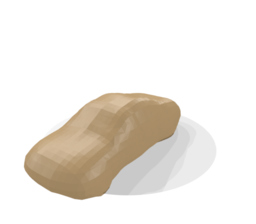
\includegraphics[width=1.75cm,trim={0.25cm 0.25cm 1.25cm 1.25cm},clip]{gfx/appendix_experiments_prior/vae_occ+sdf/sb.clean.5.large/sdf/00004}
        \end{subfigure}
        \begin{subfigure}[t]{0.115\textwidth}
            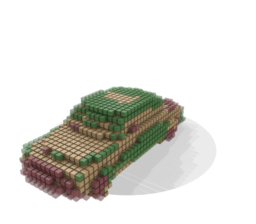
\includegraphics[width=1.75cm,trim={0.25cm 0.25cm 1.25cm 1.25cm},clip]{gfx/appendix_experiments_prior/vae_occ+sdf/sb.clean.5.large/binvox/00004}
        \end{subfigure}
        \begin{subfigure}[t]{0.115\textwidth}
            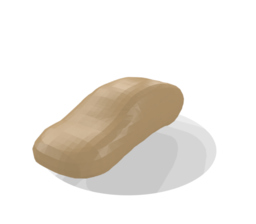
\includegraphics[width=1.75cm,trim={0.25cm 0.25cm 1.25cm 1.25cm},clip]{gfx/appendix_experiments_prior/vae_occ+sdf/sb.clean.5.large/sdf/00009}
        \end{subfigure}
        \begin{subfigure}[t]{0.115\textwidth}
            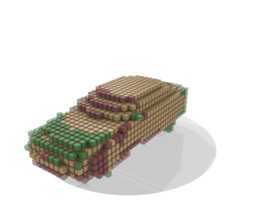
\includegraphics[width=1.75cm,trim={0.25cm 0.25cm 1.25cm 1.25cm},clip]{gfx/appendix_experiments_prior/vae_occ+sdf/sb.clean.5.large/binvox/00009}
        \end{subfigure}
        \begin{subfigure}[t]{0.115\textwidth}
            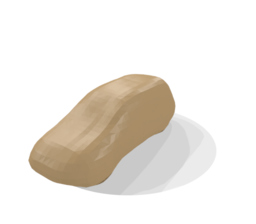
\includegraphics[width=1.75cm,trim={0.25cm 0.25cm 1.25cm 1.25cm},clip]{gfx/appendix_experiments_prior/vae_occ+sdf/sb.clean.5.large/sdf/00007}
        \end{subfigure}
        \begin{subfigure}[t]{0.115\textwidth}
            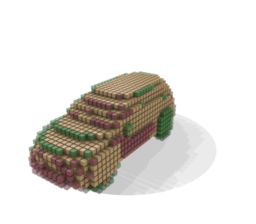
\includegraphics[width=1.75cm,trim={0.25cm 0.25cm 1.25cm 1.25cm},clip]{gfx/appendix_experiments_prior/vae_occ+sdf/sb.clean.5.large/binvox/00007}
        \end{subfigure}
        \begin{subfigure}[t]{0.115\textwidth}
            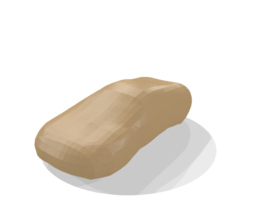
\includegraphics[width=1.75cm,trim={0.25cm 0.25cm 1.25cm 1.25cm},clip]{gfx/appendix_experiments_prior/vae_occ+sdf/sb.clean.5.large/sdf/00012}
        \end{subfigure}
        \begin{subfigure}[t]{0.115\textwidth}
            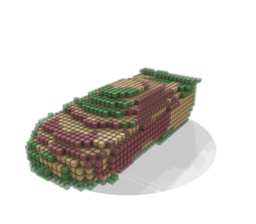
\includegraphics[width=1.75cm,trim={0.25cm 0.25cm 1.25cm 1.25cm},clip]{gfx/appendix_experiments_prior/vae_occ+sdf/sb.clean.5.large/binvox/00012}
        \end{subfigure}\\
        \begin{subfigure}[t]{0.115\textwidth}
            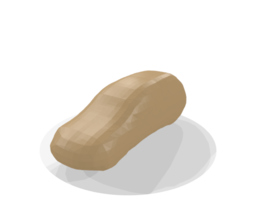
\includegraphics[width=1.75cm,trim={0.25cm 0.25cm 1.25cm 1.25cm},clip]{gfx/appendix_experiments_prior/vae_occ+sdf/sb.clean.5.large/sdf_random/00013}
        \end{subfigure}
        \begin{subfigure}[t]{0.115\textwidth}
            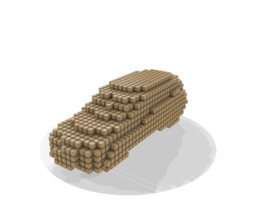
\includegraphics[width=1.75cm,trim={0.25cm 0.25cm 1.25cm 1.25cm},clip]{gfx/appendix_experiments_prior/vae_occ+sdf/sb.clean.5.large/binvox_random/00013}
        \end{subfigure}
        \begin{subfigure}[t]{0.115\textwidth}
            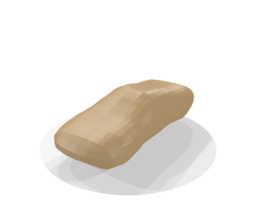
\includegraphics[width=1.75cm,trim={0.25cm 0.25cm 1.25cm 1.25cm},clip]{gfx/appendix_experiments_prior/vae_occ+sdf/sb.clean.5.large/sdf_random/00001}
        \end{subfigure}
        \begin{subfigure}[t]{0.115\textwidth}
            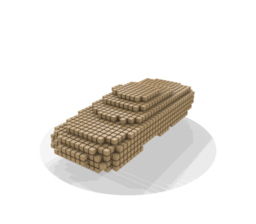
\includegraphics[width=1.75cm,trim={0.25cm 0.25cm 1.25cm 1.25cm},clip]{gfx/appendix_experiments_prior/vae_occ+sdf/sb.clean.5.large/binvox_random/00001}
        \end{subfigure}
        \begin{subfigure}[t]{0.115\textwidth}
            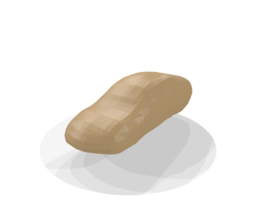
\includegraphics[width=1.75cm,trim={0.25cm 0.25cm 1.25cm 1.25cm},clip]{gfx/appendix_experiments_prior/vae_occ+sdf/sb.clean.5.large/sdf_random/00002}
        \end{subfigure}
        \begin{subfigure}[t]{0.115\textwidth}
            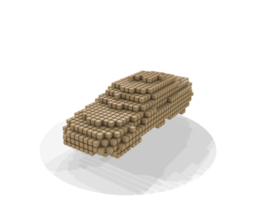
\includegraphics[width=1.75cm,trim={0.25cm 0.25cm 1.25cm 1.25cm},clip]{gfx/appendix_experiments_prior/vae_occ+sdf/sb.clean.5.large/binvox_random/00002}
        \end{subfigure}
        \begin{subfigure}[t]{0.115\textwidth}
            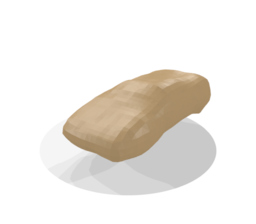
\includegraphics[width=1.75cm,trim={0.25cm 0.25cm 1.25cm 1.25cm},clip]{gfx/appendix_experiments_prior/vae_occ+sdf/sb.clean.5.large/sdf_random/00004}
        \end{subfigure}
        \begin{subfigure}[t]{0.115\textwidth}
            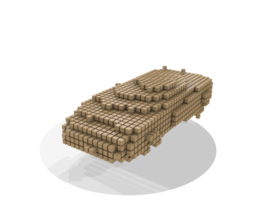
\includegraphics[width=1.75cm,trim={0.25cm 0.25cm 1.25cm 1.25cm},clip]{gfx/appendix_experiments_prior/vae_occ+sdf/sb.clean.5.large/binvox_random/00004}
        \end{subfigure}
    \end{subfigure}
    \hspace*{0cm}{\color{black!25}\rule{0.9\linewidth}{0.5px}}\\[-0.4cm]
    \hspace*{0.5cm}
    \begin{subfigure}[t]{0.035\textwidth}
        \vspace{0px}
        \rotatebox{90}{\small\VAE $Q{=}10$\hspace*{0.75cm}}
    \end{subfigure}
    \begin{subfigure}[t]{0.9\textwidth}
        \vspace{0px}
        \begin{subfigure}[t]{0.115\textwidth}
            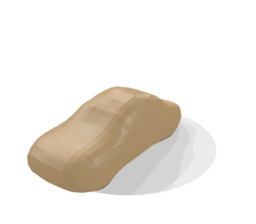
\includegraphics[width=1.75cm,trim={0.25cm 0.25cm 1.25cm 1.25cm},clip]{gfx/appendix_experiments_prior/vae_occ+sdf/sb.clean.10.large/sdf/00004}
        \end{subfigure}
        \begin{subfigure}[t]{0.115\textwidth}
            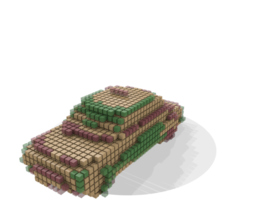
\includegraphics[width=1.75cm,trim={0.25cm 0.25cm 1.25cm 1.25cm},clip]{gfx/appendix_experiments_prior/vae_occ+sdf/sb.clean.10.large/binvox/00004}
        \end{subfigure}
        \begin{subfigure}[t]{0.115\textwidth}
            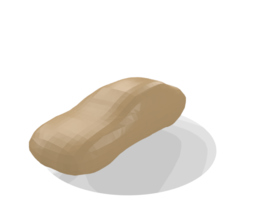
\includegraphics[width=1.75cm,trim={0.25cm 0.25cm 1.25cm 1.25cm},clip]{gfx/appendix_experiments_prior/vae_occ+sdf/sb.clean.10.large/sdf/00009}
        \end{subfigure}
        \begin{subfigure}[t]{0.115\textwidth}
            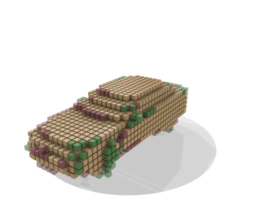
\includegraphics[width=1.75cm,trim={0.25cm 0.25cm 1.25cm 1.25cm},clip]{gfx/appendix_experiments_prior/vae_occ+sdf/sb.clean.10.large/binvox/00009}
        \end{subfigure}
        \begin{subfigure}[t]{0.115\textwidth}
            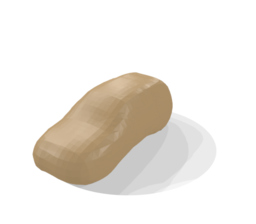
\includegraphics[width=1.75cm,trim={0.25cm 0.25cm 1.25cm 1.25cm},clip]{gfx/appendix_experiments_prior/vae_occ+sdf/sb.clean.10.large/sdf/00007}
        \end{subfigure}
        \begin{subfigure}[t]{0.115\textwidth}
            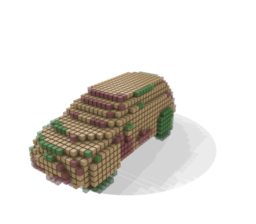
\includegraphics[width=1.75cm,trim={0.25cm 0.25cm 1.25cm 1.25cm},clip]{gfx/appendix_experiments_prior/vae_occ+sdf/sb.clean.10.large/binvox/00007}
        \end{subfigure}
        \begin{subfigure}[t]{0.115\textwidth}
            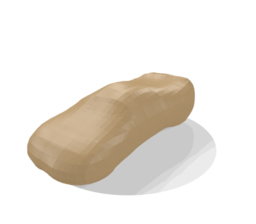
\includegraphics[width=1.75cm,trim={0.25cm 0.25cm 1.25cm 1.25cm},clip]{gfx/appendix_experiments_prior/vae_occ+sdf/sb.clean.10.large/sdf/00012}
        \end{subfigure}
        \begin{subfigure}[t]{0.115\textwidth}
            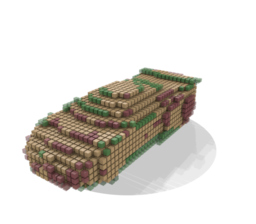
\includegraphics[width=1.75cm,trim={0.25cm 0.25cm 1.25cm 1.25cm},clip]{gfx/appendix_experiments_prior/vae_occ+sdf/sb.clean.10.large/binvox/00012}
        \end{subfigure}\\
        \begin{subfigure}[t]{0.115\textwidth}
            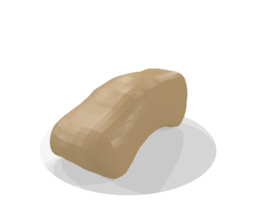
\includegraphics[width=1.75cm,trim={0.25cm 0.25cm 1.25cm 1.25cm},clip]{gfx/appendix_experiments_prior/vae_occ+sdf/sb.clean.10.large/sdf_random/00013}
        \end{subfigure}
        \begin{subfigure}[t]{0.115\textwidth}
            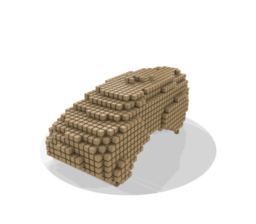
\includegraphics[width=1.75cm,trim={0.25cm 0.25cm 1.25cm 1.25cm},clip]{gfx/appendix_experiments_prior/vae_occ+sdf/sb.clean.10.large/binvox_random/00013}
        \end{subfigure}
        \begin{subfigure}[t]{0.115\textwidth}
            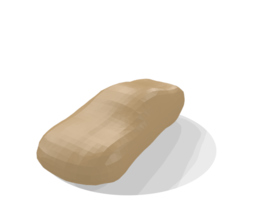
\includegraphics[width=1.75cm,trim={0.25cm 0.25cm 1.25cm 1.25cm},clip]{gfx/appendix_experiments_prior/vae_occ+sdf/sb.clean.10.large/sdf_random/00001}
        \end{subfigure}
        \begin{subfigure}[t]{0.115\textwidth}
            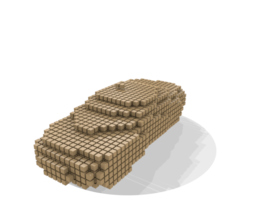
\includegraphics[width=1.75cm,trim={0.25cm 0.25cm 1.25cm 1.25cm},clip]{gfx/appendix_experiments_prior/vae_occ+sdf/sb.clean.10.large/binvox_random/00001}
        \end{subfigure}
        \begin{subfigure}[t]{0.115\textwidth}
            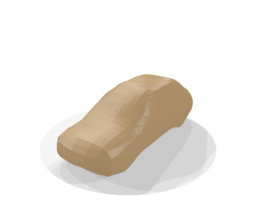
\includegraphics[width=1.75cm,trim={0.25cm 0.25cm 1.25cm 1.25cm},clip]{gfx/appendix_experiments_prior/vae_occ+sdf/sb.clean.10.large/sdf_random/00002}
        \end{subfigure}
        \begin{subfigure}[t]{0.115\textwidth}
            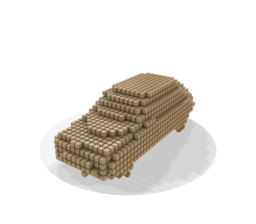
\includegraphics[width=1.75cm,trim={0.25cm 0.25cm 1.25cm 1.25cm},clip]{gfx/appendix_experiments_prior/vae_occ+sdf/sb.clean.10.large/binvox_random/00002}
        \end{subfigure}
        \begin{subfigure}[t]{0.115\textwidth}
            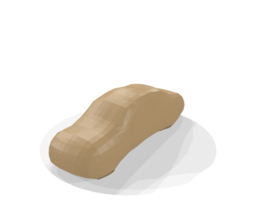
\includegraphics[width=1.75cm,trim={0.25cm 0.25cm 1.25cm 1.25cm},clip]{gfx/appendix_experiments_prior/vae_occ+sdf/sb.clean.10.large/sdf_random/00004}
        \end{subfigure}
        \begin{subfigure}[t]{0.115\textwidth}
            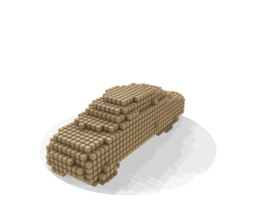
\includegraphics[width=1.75cm,trim={0.25cm 0.25cm 1.25cm 1.25cm},clip]{gfx/appendix_experiments_prior/vae_occ+sdf/sb.clean.10.large/binvox_random/00004}
        \end{subfigure}
    \end{subfigure}
    \hspace*{0cm}{\color{black!25}\rule{0.9\linewidth}{0.5px}}\\[-0.4cm]
    \hspace*{0.5cm}
    \begin{subfigure}[t]{0.035\textwidth}
        \vspace{0px}
        \rotatebox{90}{\small\VAE $Q{=}25$\hspace*{0.75cm}}
    \end{subfigure}
    \begin{subfigure}[t]{0.9\textwidth}
        \vspace{0px}
        \begin{subfigure}[t]{0.115\textwidth}
            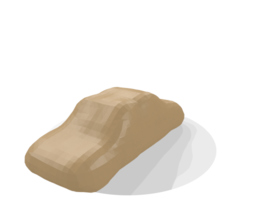
\includegraphics[width=1.75cm,trim={0.25cm 0.25cm 1.25cm 1.25cm},clip]{gfx/appendix_experiments_prior/vae_occ+sdf/sb.clean.25.large/sdf/00004}
        \end{subfigure}
        \begin{subfigure}[t]{0.115\textwidth}
            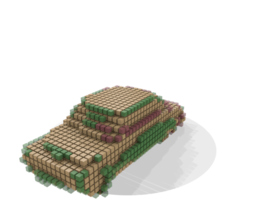
\includegraphics[width=1.75cm,trim={0.25cm 0.25cm 1.25cm 1.25cm},clip]{gfx/appendix_experiments_prior/vae_occ+sdf/sb.clean.25.large/binvox/00004}
        \end{subfigure}
        \begin{subfigure}[t]{0.115\textwidth}
            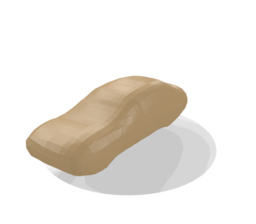
\includegraphics[width=1.75cm,trim={0.25cm 0.25cm 1.25cm 1.25cm},clip]{gfx/appendix_experiments_prior/vae_occ+sdf/sb.clean.25.large/sdf/00009}
        \end{subfigure}
        \begin{subfigure}[t]{0.115\textwidth}
            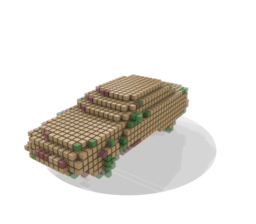
\includegraphics[width=1.75cm,trim={0.25cm 0.25cm 1.25cm 1.25cm},clip]{gfx/appendix_experiments_prior/vae_occ+sdf/sb.clean.25.large/binvox/00009}
        \end{subfigure}
        \begin{subfigure}[t]{0.115\textwidth}
            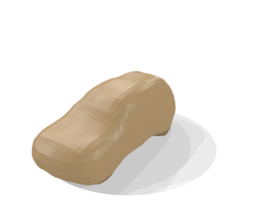
\includegraphics[width=1.75cm,trim={0.25cm 0.25cm 1.25cm 1.25cm},clip]{gfx/appendix_experiments_prior/vae_occ+sdf/sb.clean.25.large/sdf/00007}
        \end{subfigure}
        \begin{subfigure}[t]{0.115\textwidth}
            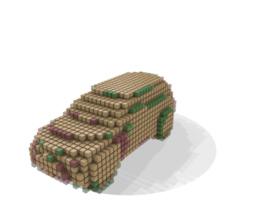
\includegraphics[width=1.75cm,trim={0.25cm 0.25cm 1.25cm 1.25cm},clip]{gfx/appendix_experiments_prior/vae_occ+sdf/sb.clean.25.large/binvox/00007}
        \end{subfigure}
        \begin{subfigure}[t]{0.115\textwidth}
            \includegraphics[width=1.75cm,trim={0.25cm 0.25cm 1.25cm 1.25cm},clip]{gfx/appendix_experiments_prior/vae_occ+sdf/sb.clean.25.large/sdf/00012}
        \end{subfigure}
        \begin{subfigure}[t]{0.115\textwidth}
            \includegraphics[width=1.75cm,trim={0.25cm 0.25cm 1.25cm 1.25cm},clip]{gfx/appendix_experiments_prior/vae_occ+sdf/sb.clean.25.large/binvox/00012}
        \end{subfigure}\\
        \begin{subfigure}[t]{0.115\textwidth}
            \includegraphics[width=1.75cm,trim={0.25cm 0.25cm 1.25cm 1.25cm},clip]{gfx/appendix_experiments_prior/vae_occ+sdf/sb.clean.25.large/sdf_random/00013}
        \end{subfigure}
        \begin{subfigure}[t]{0.115\textwidth}
            \includegraphics[width=1.75cm,trim={0.25cm 0.25cm 1.25cm 1.25cm},clip]{gfx/appendix_experiments_prior/vae_occ+sdf/sb.clean.25.large/binvox_random/00013}
        \end{subfigure}
        \begin{subfigure}[t]{0.115\textwidth}
            \includegraphics[width=1.75cm,trim={0.25cm 0.25cm 1.25cm 1.25cm},clip]{gfx/appendix_experiments_prior/vae_occ+sdf/sb.clean.25.large/sdf_random/00001}
        \end{subfigure}
        \begin{subfigure}[t]{0.115\textwidth}
            \includegraphics[width=1.75cm,trim={0.25cm 0.25cm 1.25cm 1.25cm},clip]{gfx/appendix_experiments_prior/vae_occ+sdf/sb.clean.25.large/binvox_random/00001}
        \end{subfigure}
        \begin{subfigure}[t]{0.115\textwidth}
            \includegraphics[width=1.75cm,trim={0.25cm 0.25cm 1.25cm 1.25cm},clip]{gfx/appendix_experiments_prior/vae_occ+sdf/sb.clean.25.large/sdf_random/00002}
        \end{subfigure}
        \begin{subfigure}[t]{0.115\textwidth}
            \includegraphics[width=1.75cm,trim={0.25cm 0.25cm 1.25cm 1.25cm},clip]{gfx/appendix_experiments_prior/vae_occ+sdf/sb.clean.25.large/binvox_random/00002}
        \end{subfigure}
        \begin{subfigure}[t]{0.115\textwidth}
            \includegraphics[width=1.75cm,trim={0.25cm 0.25cm 1.25cm 1.25cm},clip]{gfx/appendix_experiments_prior/vae_occ+sdf/sb.clean.25.large/sdf_random/00004}
        \end{subfigure}
        \begin{subfigure}[t]{0.115\textwidth}
            \includegraphics[width=1.75cm,trim={0.25cm 0.25cm 1.25cm 1.25cm},clip]{gfx/appendix_experiments_prior/vae_occ+sdf/sb.clean.25.large/binvox_random/00004}
        \end{subfigure}
    \end{subfigure}
    \hspace*{0cm}{\color{black!25}\rule{0.9\linewidth}{0.5px}}\\[-0.4cm]
    \hspace*{0.5cm}
    \begin{subfigure}[t]{0.035\textwidth}
        \vspace{0px}
        \rotatebox{90}{\small\PPCA $Q{=}10$\hspace*{0.75cm}}
    \end{subfigure}
    \begin{subfigure}[t]{0.9\textwidth}
        \vspace{0px}
        \begin{subfigure}[t]{0.115\textwidth}
            \includegraphics[width=1.75cm,trim={0.25cm 0.25cm 1.25cm 1.25cm},clip]{gfx/appendix_experiments_prior/ppca_occ+sdf/sb.clean.10.large/sdf/00004}
        \end{subfigure}
        \begin{subfigure}[t]{0.115\textwidth}
            \includegraphics[width=1.75cm,trim={0.25cm 0.25cm 1.25cm 1.25cm},clip]{gfx/appendix_experiments_prior/ppca_occ+sdf/sb.clean.10.large/binvox/00004}
        \end{subfigure}
        \begin{subfigure}[t]{0.115\textwidth}
            \includegraphics[width=1.75cm,trim={0.25cm 0.25cm 1.25cm 1.25cm},clip]{gfx/appendix_experiments_prior/ppca_occ+sdf/sb.clean.10.large/sdf/00009}
        \end{subfigure}
        \begin{subfigure}[t]{0.115\textwidth}
            \includegraphics[width=1.75cm,trim={0.25cm 0.25cm 1.25cm 1.25cm},clip]{gfx/appendix_experiments_prior/ppca_occ+sdf/sb.clean.10.large/binvox/00009}
        \end{subfigure}
        \begin{subfigure}[t]{0.115\textwidth}
            \includegraphics[width=1.75cm,trim={0.25cm 0.25cm 1.25cm 1.25cm},clip]{gfx/appendix_experiments_prior/ppca_occ+sdf/sb.clean.10.large/sdf/00007}
        \end{subfigure}
        \begin{subfigure}[t]{0.115\textwidth}
            \includegraphics[width=1.75cm,trim={0.25cm 0.25cm 1.25cm 1.25cm},clip]{gfx/appendix_experiments_prior/ppca_occ+sdf/sb.clean.10.large/binvox/00007}
        \end{subfigure}
        \begin{subfigure}[t]{0.115\textwidth}
            \includegraphics[width=1.75cm,trim={0.25cm 0.25cm 1.25cm 1.25cm},clip]{gfx/appendix_experiments_prior/ppca_occ+sdf/sb.clean.10.large/sdf/00012}
        \end{subfigure}
        \begin{subfigure}[t]{0.115\textwidth}
            \includegraphics[width=1.75cm,trim={0.25cm 0.25cm 1.25cm 1.25cm},clip]{gfx/appendix_experiments_prior/ppca_occ+sdf/sb.clean.10.large/binvox/00012}
        \end{subfigure}\\
        \begin{subfigure}[t]{0.115\textwidth}
            \includegraphics[width=1.75cm,trim={0.25cm 0.25cm 1.25cm 1.25cm},clip]{gfx/appendix_experiments_prior/ppca_occ+sdf/sb.clean.10.large/sdf_random/00013}
        \end{subfigure}
        \begin{subfigure}[t]{0.115\textwidth}
            \includegraphics[width=1.75cm,trim={0.25cm 0.25cm 1.25cm 1.25cm},clip]{gfx/appendix_experiments_prior/ppca_occ+sdf/sb.clean.10.large/binvox_random/00013}
        \end{subfigure}
        \begin{subfigure}[t]{0.115\textwidth}
            \includegraphics[width=1.75cm,trim={0.25cm 0.25cm 1.25cm 1.25cm},clip]{gfx/appendix_experiments_prior/ppca_occ+sdf/sb.clean.10.large/sdf_random/00001}
        \end{subfigure}
        \begin{subfigure}[t]{0.115\textwidth}
            \includegraphics[width=1.75cm,trim={0.25cm 0.25cm 1.25cm 1.25cm},clip]{gfx/appendix_experiments_prior/ppca_occ+sdf/sb.clean.10.large/binvox_random/00001}
        \end{subfigure}
        \begin{subfigure}[t]{0.115\textwidth}
            \includegraphics[width=1.75cm,trim={0.25cm 0.25cm 1.25cm 1.25cm},clip]{gfx/appendix_experiments_prior/ppca_occ+sdf/sb.clean.10.large/sdf_random/00002}
        \end{subfigure}
        \begin{subfigure}[t]{0.115\textwidth}
            \includegraphics[width=1.75cm,trim={0.25cm 0.25cm 1.25cm 1.25cm},clip]{gfx/appendix_experiments_prior/ppca_occ+sdf/sb.clean.10.large/binvox_random/00002}
        \end{subfigure}
        \begin{subfigure}[t]{0.115\textwidth}
            \includegraphics[width=1.75cm,trim={0.25cm 0.25cm 1.25cm 1.25cm},clip]{gfx/appendix_experiments_prior/ppca_occ+sdf/sb.clean.10.large/sdf_random/00004}
        \end{subfigure}
        \begin{subfigure}[t]{0.115\textwidth}
            \includegraphics[width=1.75cm,trim={0.25cm 0.25cm 1.25cm 1.25cm},clip]{gfx/appendix_experiments_prior/ppca_occ+sdf/sb.clean.10.large/binvox_random/00004}
        \end{subfigure}
    \end{subfigure}
    \caption{{\bf Additional Qualitative Results.} Reconstruction performance and random samples for our \VAE shape prior in comparison with a \PPCA shape prior for different sizes of the latent space $Q$. In each case, we show reconstructions in the top row and random samples in the bottom row; for occupancy grids we also show false positives ({\color{rred}red}) and false negatives ({\color{rgreen}green}).}
    \label{fig:appendix-experiments-prior}
\end{figure*}
\begin{table}
    \centering
    \vspace*{-0.25cm}
    \begin{subfigure}[t]{0.49\textwidth}
    	\vspace{0px}
        % clean
        % -----
        % [Data] set: validation.json
        % [Data] N: 1950
        % [Data] pixels: 31104
        % [Data] points: 411.713333333
        % [Data] occupied: 3525
        % [Data] observed points: 331.593333333
        % [Data] observed space: 2190.67692308
        % [Data] observed total: 2522.27025641
        % [Data] observed invalid: 24.0307692308
        % [Data] set: training_prior.json
        % [Data] N: 14640
        % [Data] pixels: 31104
        % [Data] points: 407.848838798
        % [Data] occupied: 3522
        % [Data] observed points: 329.771857923
        % [Data] observed space: 2193.04344262
        % [Data] observed total: 2522.8135929
        % [Data] observed invalid: 24.9206967213
        % [Data] set: training_inference.json
        % [Data] N: 14640
        % [Data] pixels: 31104
        % [Data] points: 410.855874317
        % [Data] occupied: 3574
        % [Data] observed points: 331.223702186
        % [Data] observed space: 2200.80642077
        % [Data] observed total: 2532.03224044
        % [Data] observed invalid: 27.4879098361
        % noisy
        % -----
        % [Data] set: training_inference.json
        % [Data] N: 14640
        % [Data] pixels: 31104
        % [Data] points: 106.733538251
        % [Data] occupied: 3574
        % [Data] observed points: 100.450819672
        % [Data] observed space: 1507.3431694
        % [Data] observed total: 1607.79535519
        % [Data] observed invalid: 143.542076503
        % [Data] set: validation.json
        % [Data] N: 1950
        % [Data] pixels: 31104
        % [Data] points: 106.267692308
        % [Data] occupied: 3525
        % [Data] observed points: 100.188205128
        % [Data] observed space: 1483.26205128
        % [Data] observed total: 1583.45025641
        % [Data] observed invalid: 136.838461538
        % [Data] set: training_prior.json
        % [Data] N: 14640
        % [Data] pixels: 31104
        % [Data] points: 105.880737705
        % [Data] occupied: 3522
        % [Data] observed points: 99.7855874317
        % [Data] observed space: 1499.75751366
        % [Data] observed total: 1599.54357923
        % [Data] observed invalid: 142.554098361
        
        {\small
        \begin{tabularx}{1\textwidth}{|X|c|c|}
            \hline
            \clean and \noisy & \clean & \noisy\\
            \hline
            \#Models (Prior / Inference / Val) & \multicolumn{2}{c|}{325 / 1464 / 1464}\\ % = 3253
            \#Samples (Prior / Inference / Val) & \multicolumn{2}{c|}{1950 / 14640 / 1464}\\
            \hline
            Avg. \#Points & 411 & 106\\
            \% Observed / Free Space Voxels & 1.06 / 7.04 & 0.32 / 4.8\\
            %\% Free Space Voxels & 7.04 & 4.8\\
            \% Invalid Free Space Voxels & 0.078 & 0.44\\
            \hline
        \end{tabularx}
        }
        % training
        % --------
        % [Data] N: 7140
        % [Data] pixels: 31104
        % [Data] points: 135.218907563
        % [Data] observed frames: 7
        % [Data] observed points: 135
        % [Data] observed points (combined GT): 855
        % [Data] observed points voxels: 95.9831932773
        % [Data] observed points voxels (combined GT): 330.200840336
        % [Data] observed space voxels: 1084.93837535
        % [Data] observed total voxels: 1180.92156863
        % [Data] observed invalid space voxels: 84.0274859944
        % validation
        % ----------
        % [Data] N: 7118
        % [Data] pixels: 31104
        % [Data] points: 128.333520652
        % [Data] observed frames: 6
        % [Data] observed points: 128
        % [Data] observed points (combined GT): 597
        % [Data] observed points voxels: 89.0772688958
        % [Data] observed points voxels (combined GT): 303.195420062
        % [Data] observed space voxels: 975.978645687
        % [Data] observed total voxels: 1065.05591458
        % [Data] observed invalid space voxels: 88.295123279
        
        \vspace*{0.05cm}
        {\small
        	\begin{tabularx}{1\textwidth}{|X|c|c|}
        		\hline
        		KITTI
        		& Training
        		& Validation\\
        		\hline
        		\#Samples & 7140 & 7118\\
        		Avg. \#Points & 135 & 128\\
        		\% Observed / Free Space Voxels & 0.31 / 3.49 & 0.29 / \green{3.2}\\
        		%\% Free Space Voxels & 3.49 & 3.42\\
        		%Invalid Free Space Voxels* in \% & 0.27 & 0.28\\
        		%\hline
        		%Ground Truth Points & 855 & 597\\
        		%Ground Truth Frames & 7 & 6\\
        		\hline
        	\end{tabularx}
        }
    \end{subfigure}
    \begin{subfigure}[t]{0.49\textwidth}
    	\vspace{0px}
%		bathtub:
%    	[Data] set: training_inference.json
%    	[Data] N: 700
%    	[Data] pixels: 32768
%    	[Data] points: 618.8742857142857
%    	[Data] occupied: 1084
%    	[Data] observed points: 204.52
%    	[Data] observed space: 1226.44
%    	[Data] observed total: 1430.96
%    	[Data] observed invalid: 64.2285714286
%    	[Data] set: validation.json
%    	[Data] N: 150
%    	[Data] pixels: 32768
%    	[Data] points: 593.44
%    	[Data] occupied: 967
%    	[Data] observed points: 198.70666666666668
%    	[Data] observed space: 1213.3666666666666
%    	[Data] observed total: 1412.07333333
%    	[Data] observed invalid: 57.5466666667
%    	[Data] set: training_prior.json
%    	[Data] N: 700
%    	[Data] pixels: 32768
%    	[Data] points: 636.45
%    	[Data] occupied: 1085
%    	[Data] observed points: 209.44
%    	[Data] observed space: 1252.6128571428571
%    	[Data] observed total: 1462.05285714
%    	[Data] observed invalid: 66.5385714286
%		dresser:
%		[Data] set: training_prior.json
%		[Data] N: 1280
%		[Data] pixels: 32768
%		[Data] points: 1394.06796875
%		[Data] occupied: 1916
%		[Data] observed points: 411.1375
%		[Data] observed space: 2746.1984375
%		[Data] observed total: 3157.3359375
%		[Data] observed invalid: 81.19453125
%		[Data] set: validation.json
%		[Data] N: 280
%		[Data] pixels: 32768
%		[Data] points: 1348.8285714285714
%		[Data] occupied: 2020
%		[Data] observed points: 409.2214285714286
%		[Data] observed space: 2736.582142857143
%		[Data] observed total: 3145.80357143
%		[Data] observed invalid: 99.1392857143
%		[Data] set: training_inference.json
%		[Data] N: 1280
%		[Data] pixels: 32768
%		[Data] points: 1475.1546875
%		[Data] occupied: 2071
%		[Data] observed points: 433.32421875
%		[Data] observed space: 2872.15
%		[Data] observed total: 3305.47421875
%		[Data] observed invalid: 90.4984375
%		monitor:
%		[Data] set: training_inference.json
%		[Data] N: 1524
%		[Data] pixels: 32768
%		[Data] points: 1057.268372703412
%		[Data] occupied: 1164
%		[Data] observed points: 372.9665354330709
%		[Data] observed space: 3028.1115485564305
%		[Data] observed total: 3401.07808399
%		[Data] observed invalid: 101.791338583
%		[Data] set: training_prior.json
%		[Data] N: 1524
%		[Data] pixels: 32768
%		[Data] points: 1066.755905511811
%		[Data] occupied: 1236
%		[Data] observed points: 374.28477690288713
%		[Data] observed space: 2931.3930446194227
%		[Data] observed total: 3305.67782152
%		[Data] observed invalid: 110.317585302
%		[Data] set: validation.json
%		[Data] N: 336
%		[Data] pixels: 32768
%		[Data] points: 1113.172619047619
%		[Data] occupied: 1233
%		[Data] observed points: 373.9136904761905
%		[Data] observed space: 2914.6488095238096
%		[Data] observed total: 3288.5625
%		[Data] observed invalid: 97.8898809524
%		nighstand:
%		[Data] set: validation.json
%		[Data] N: 280
%		[Data] pixels: 32768
%		[Data] points: 1502.107142857143
%		[Data] occupied: 2546
%		[Data] observed points: 474.1142857142857
%		[Data] observed space: 3169.9142857142856
%		[Data] observed total: 3644.02857143
%		[Data] observed invalid: 193.632142857
%		[Data] set: training_inference.json
%		[Data] N: 1280
%		[Data] pixels: 32768
%		[Data] points: 1472.47109375
%		[Data] occupied: 2344
%		[Data] observed points: 464.253125
%		[Data] observed space: 3075.828125
%		[Data] observed total: 3540.08125
%		[Data] observed invalid: 168.1203125
%		[Data] set: training_prior.json
%		[Data] N: 1280
%		[Data] pixels: 32768
%		[Data] points: 1465.19296875
%		[Data] occupied: 2295
%		[Data] observed points: 461.2640625
%		[Data] observed space: 3098.29609375
%		[Data] observed total: 3559.56015625
%		[Data] observed invalid: 178.5890625
%		sofa:
%		[Data] set: training_inference.json
%		[Data] N: 1755
%		[Data] pixels: 32768
%		[Data] points: 587.757264957265
%		[Data] occupied: 1077
%		[Data] observed points: 207.43817663817663
%		[Data] observed space: 1418.0962962962963
%		[Data] observed total: 1625.53447293
%		[Data] observed invalid: 76.4643874644
%		[Data] set: training_prior.json
%		[Data] N: 1755
%		[Data] pixels: 32768
%		[Data] points: 592.8398860398861
%		[Data] occupied: 1073
%		[Data] observed points: 209.92934472934473
%		[Data] observed space: 1440.480341880342
%		[Data] observed total: 1650.40968661
%		[Data] observed invalid: 77.29002849
%		[Data] set: validation.json
%		[Data] N: 390
%		[Data] pixels: 32768
%		[Data] points: 643.2666666666667
%		[Data] occupied: 1128
%		[Data] observed points: 226.63333333333333
%		[Data] observed space: 1520.7282051282052
%		[Data] observed total: 1747.36153846
%		[Data] observed invalid: 80.0435897436
% 		toilet:
%		[Data] set: training_inference.json
%		[Data] N: 1393
%		[Data] pixels: 32768
%		[Data] points: 998.0308686288586
%		[Data] occupied: 1618
%		[Data] observed points: 356.02153625269204
%		[Data] observed space: 2407.643216080402
%		[Data] observed total: 2763.66475233
%		[Data] observed invalid: 103.513280689
%		[Data] set: training_prior.json
%		[Data] N: 1393
%		[Data] pixels: 32768
%		[Data] points: 1005.1399856424982
%		[Data] occupied: 1593
%		[Data] observed points: 355.5362526920316
%		[Data] observed space: 2396.049533381192
%		[Data] observed total: 2751.58578607
%		[Data] observed invalid: 106.465183058
%		[Data] set: validation.json
%		[Data] N: 308
%		[Data] pixels: 32768
%		[Data] points: 1009.9285714285714
%		[Data] occupied: 1676
%		[Data] observed points: 360.1233766233766
%		[Data] observed space: 2445.103896103896
%		[Data] observed total: 2805.22727273
%		[Data] observed invalid: 106.863636364
%		bdmnsf:
%		[Data] set: training_inference
%		[Data] N: 7932
%		[Data] pixels: 32768
%		[Data] points: 1038.731845688351
%		[Data] occupied: 2357.516515380736
%		[Data] observed points: 342.97226424609175
%		[Data] observed space: 2386.4558749369644
%		[Data] observed total: 2729.42813918
%		[Data] observed invalid: 110.759707514
%		[Data] set: training_prior
%		[Data] N: 7932
%		[Data] pixels: 32768
%		[Data] points: 1030.2192385274836
%		[Data] occupied: 2366.558623298033
%		[Data] observed points: 340.0630358043369
%		[Data] observed space: 2356.399899142713
%		[Data] observed total: 2696.46306102
%		[Data] observed invalid: 115.949445285
%		[Data] set: validation
%		[Data] N: 1744
%		[Data] pixels: 32768
%		[Data] points: 1045.4334862385322
%		[Data] occupied: 2433.5424311926604
%		[Data] observed points: 345.22935779816515
%		[Data] observed space: 2386.079128440367
%		[Data] observed total: 2731.30848624
%		[Data] observed invalid: 114.655389908
%		
    	{\small
   		\begin{tabularx}{1\textwidth}{|X|c|c|c|}
   			\hline
   			ModelNet& Prior & Inference & Val\\
   			\hline
   			\#Models / \#Samples&&&\\
   			\quad bathtub & \green{70 / 700} & \green{70 / 700} & \green{15 / 150}\\
   			\quad dresser & \green{128 / 1280} & \green{128 / 1280} & \green{28 / 280}\\
   			\quad monitor & \green{254 / 1524} & \green{254 / 1524} & \green{56 / 336}\\
   			\quad nightstand & \green{128 / 1280} & \green{128 / 1280} & \green{28 / 280}\\
   			\quad sofa & \green{351 / 1755} & \green{351 / 1755} & \green{78 / 390}\\
   			\quad toilet & \green{199 / 1393} & \green{199 / 1393} & \green{44 / 308}\\
   			\hline
   			Avg. \#Points & \green{1030} & \green{1038} & \green{1045}\\
   			\% Observed / Free Space Voxels & \green{1.04 / 7.28} & \green{1.04 / 7.19} & \green{1.05 / 7.28}\\
   			\hline
   		\end{tabularx}
    	}
    \end{subfigure}
    \caption{{\bf Dataset Statistics.} Key statistics of the synthetic datasets, \clean, \noisy (derived from ShapeNet \cite{Chang2015ARXIV}) and ModelNet \cite{Wu2015CVPR} as well as the dataset extracted from KITTI \cite{Geiger2012CVPR}.}
    \label{table:appendix-experiments-data}
    \vspace*{-0.25cm}
\end{table}

\boldparagraph{Discussion}
%
In Figure \ref{fig:appendix-experiments-data}, we show additional qualitative examples of the constructed datasets. As can be seen, \clean and \noisy show quite some variation in the type of cars included, as well as the generated observations -- \clean, however, is considerable easier than \noisy. This is mainly due to the sparse and very noisy observations generated for \noisy. However, when considering KITTI, we see that real world data is very sparse and noisy by nature. We also see that the ground truth derived on KITTI is not perfect: for some samples, ground truth could not be generated; for others, the future / past frames do not contain novel viewpoints; \green{or accumulated points do clearly not belong to the same car. On ModelNet, we observe that other object categories exhibit significantly more variations compared to ShapeNet's (simplified) cars; additionally thin structures contribute to the difficulty of ModelNet for 3D shape completion. Finally, Table \ref{table:appendix-experiments-data} summarizes key statistics of the created datasets.}

\section{Architecture}
\label{sec:appendix-architecture}

Throughout our experiments, we found both the architecture and the shape representation to have significant influence on our results. On ShapeNet and KITTI, we used a shallow architecture where both encoder and decoder consist of three convolutional stages (no bias term) including $\text{ReLU}$ non-linearities and batch normalization. We use $3^3$ kernels and apply max pooling after each stage; specifically using window sizes $2\times 3 \times 2$ (first two stages) and $3^3$ (final stage). The special windows sizes for the max pooling layers are motivated by our resolution of $24 \times 54 \times 24$. \green{On ModelNet, we used four stages with window size $2^2$ for pooling.} We also experimented with deeper architectures as well as different pooling schemes. We found that deeper architectures do not necessarily improve performance; \green{specifically we assume that the low-dimensional bottleneck ($Q = 10$ for ShapeNet/KITTI and $Q = 25$ or $Q = 100$ for ModelNet) prevents deeper architectures to result in a significant increase in performance.}
%Additionally, our shapes have been simplified such that small details have been removed prior to training.
%Our pooling scheme reduces the input to a $2^3$ cube; using slightly different pooling will increase the smallest resolution, leading to a significant increase in the number of parameters (\eg, using $2^3$ pooling instead of $3^3$ leads to $96 \cdot 3^3 = 2592$ values instead of $96 \times 2^3 = 786$ values right before the fully connected layers), while not increasing performance.
Overall, the used architecture results in a lightweight but well-performing model.

For cars on ShapeNet, we also found the shape representation to have a significant influence on training. For example, occupancy is considerably easier to learn than SDFs. We assume that both the scale/range and the loss used for predicting SDFs plays an important role; therefore, motivated by work in depth estimation \cite{Eigen2015ICCV,Eigen2014NIPS,Laina2016THREEDV}, we transformed the SDFs using $\sign(y_i)\log(1 + |y_i|)$ for $y_i \in \mathbb{R}$. We found this transformation and the combination with occupancy (\ie, predicting both in separate channels) to aid training and result in reasonable shape priors. Alternatively, we tried splitting the SDFs into positive and negative parts (in separate channels), and transforming them separately using $\log(\epsilon + y_i)$ for $y_i \in \mathbb{R}_+$ and small $\epsilon \in (0.00001, 0.01)$. However, we assume that the increased scale (\eg, for $\epsilon = 0.00001$ and $\max(y_i) = 12$ a range of roughly $(-11.51, 2.49)$) in combination with the sum-of-squared error makes training harder. Finally, we also considered truncated SDFs, \ie, truncating the values $y_i$ above a threshold (\eg $5$); however, this did not have a significant effect on training. Overall, the combination of transformed SDFs and occupancy was easiest to train.

\section{Training}
\label{sec:appendix-training}

\green{As mentioned in the main paper, we trained all our models using stochastic gradient descent (SGD) with momentum and weight decay. We initialized all weights using a standard Gaussian with standard deviation $0.02$. For the shape prior, \ie, training the recognition model $q(z|x)$ and the generative model $p(x|z)$, learning rate, momentum and weight decay were set to $10^{-7}$, $0.5$ and $10^{-6}$, respectively. We trained for $200$ epochs with batch size $16$ and decayed learning rate and momentum by factors $0.95$ and $1.025$ every $500$ iterations until reaching $10^{-14}$ and $0.9$, respectively. On ModelNet (where only occupancy grids are used), we found that a class-weighted binary cross-entropy error (weights $0.9$ and $1.1$ for unoccupied and occupied voxels, respectively) to help training. Furthermore, we used an initial learning rate of $10^{-6}$ and a decay factor of $1.04$ for the momentum parameter -- every $100$ iterations. For shape inference, \ie, training the encoder $z(x;w)$, we used the same strategy, but trained for only $50$ epochs with higher learning rate and momentum decay factors ($0.9$ and $1.1$, respectively). The supervised baseline was trained using the same strategy as the shape prior. For the maximum likelihood baseline, we also employed SGD starting with $z = 0$ for a maximum of $5000$ iterations (per sample) or until the change in objective drops below $0.001$. Initial learning and momentum were set to $0.05$ and $0.5$, respectively; both were decayed every $50$ iterations using factors $0.85$ and $1.04$, respectively.}

\section{Evaluation}
\label{sec:appendix-evaluation}

For evaluation we consider mesh-to-mesh or mesh-to-point distances to compute accuracy (\Acc) and completeness (\Compl). For computing the distance of a reconstructed mesh to a target mesh (\ie, \Acc), we randomly sample 10k points on the reconstructed mesh. This is done by first computing the area of each face and then sampling points proportionally to a face's area. This ensures that the sampled points cover the full mesh, \ie the points are uniformly distributed over the reconstructed mesh. We found that $10k$ points provide sufficient accuracy compared to deterministically sampling the mesh (\cf \cite{Jensen2014CVPR}). We then compute the distance of each point to the nearest face of the target mesh and average these distances. Similarly, we can compute completeness. On KITTI, completeness can be obtained by directly computing point-to-face distances for the ground truth points.

\section{Baselines}
\label{sec:appendix-baselines}

\begin{figure*}
    \centering
    \vspace*{-0.25cm}
    \begin{subfigure}[t]{0.02\textwidth}
        \vspace{0px}
        \rotatebox{90}{\small\clean\hspace*{0.25cm}}
    \end{subfigure}
    \begin{subfigure}[t]{0.1\textwidth}
        \vspace{0px}
        \centering
        \small Input\\
        \includegraphics[width=1.75cm,trim={0.5cm 0.75cm 1.5cm 1.5cm},clip]{gfx/experiments_data/clean*/points/00002}
    \end{subfigure}
    \begin{subfigure}[t]{0.1\textwidth}
        \vspace{0px}
        \centering
        \small\ML\\
        \includegraphics[width=1.75cm,trim={0.5cm 0.75cm 1.5cm 1.5cm},clip]{gfx/experiments_shapenet_kitti/vae_occ+sdf_ml/sb.clean.10.large.const15*/sdf_points/00002}
    \end{subfigure}
    \begin{subfigure}[t]{0.1\textwidth}
        \vspace{0px}
        \centering
        \small\cite{Engelmann2016GCPR}\\
        \includegraphics[width=1.75cm,trim={0.5cm 0.75cm 1.5cm 1.5cm},clip]{gfx/experiments_shapenet_kitti/engelmann2016/clean*/sdf_points/00002}
    \end{subfigure}
    \begin{subfigure}[t]{0.1\textwidth}
        \vspace{0px}
        \centering
        \small\AML\\
        \includegraphics[width=1.75cm,trim={0.5cm 0.75cm 1.5cm 1.5cm},clip]{gfx/experiments_shapenet_kitti/vae_occ+sdf_aml/sb.clean.10.large.const15*/sdf_points/00002}
    \end{subfigure}
    \begin{subfigure}[t]{0.1\textwidth}
        \vspace{0px}
        \centering
        \small\AML\\
        \includegraphics[width=1.75cm,trim={0.5cm 0.75cm 1.5cm 1.5cm},clip]{gfx/experiments_shapenet_kitti/vae_occ+sdf_aml/sb.clean.10.large.const15/binvox_points/00002}
    \end{subfigure}
    \begin{subfigure}[t]{0.1\textwidth}
        \vspace{0px}
        \centering
        \small\Sup\\
        \includegraphics[width=1.75cm,trim={0.5cm 0.75cm 1.5cm 1.5cm},clip]{gfx/experiments_shapenet_kitti/vae_occ+sdf_sup/sb.clean.10.large*/sdf_points/00002}
    \end{subfigure}
    \begin{subfigure}[t]{0.1\textwidth}
        \vspace{0px}
        \centering
        \small\Sup\\
        \includegraphics[width=1.75cm,trim={0.5cm 0.75cm 1.5cm 1.5cm},clip]{gfx/experiments_shapenet_kitti/vae_occ+sdf_sup/sb.clean.10.large/binvox_points/00002}
    \end{subfigure}
    \begin{subfigure}[t]{0.1\textwidth}
        \vspace{0px}
        \centering
        \small GT\\
        \includegraphics[width=1.75cm,trim={0.5cm 0.75cm 1.5cm 1.5cm},clip]{gfx/experiments_data/clean*/simplified/00002}
    \end{subfigure}
    \begin{subfigure}[t]{0.1\textwidth}
        \vspace{0px}
        \centering
        \small GT\\
        \includegraphics[width=1.75cm,trim={0.5cm 0.75cm 1.5cm 1.5cm},clip]{gfx/experiments_data/clean/voxelized/00002}
    \end{subfigure}\\
    % -------------------------------------------------------------------------------------------------
    % -------------------------------------------------------------------------------------------------
    \begin{subfigure}[t]{0.02\textwidth}
        \vspace{0px}
        \rotatebox{90}{\small\clean\hspace*{0.25cm}}
    \end{subfigure}
    \begin{subfigure}[t]{0.1\textwidth}
        \vspace{0px}
        \centering
        \includegraphics[width=1.75cm,trim={0.5cm 0.75cm 1.5cm 1.5cm},clip]{gfx/experiments_data/clean*/points/00007}
    \end{subfigure}
    \begin{subfigure}[t]{0.1\textwidth}
        \vspace{0px}
        \centering
        \includegraphics[width=1.75cm,trim={0.5cm 0.75cm 1.5cm 1.5cm},clip]{gfx/experiments_shapenet_kitti/vae_occ+sdf_ml/sb.clean.10.large.const15*/sdf_points/00007}
    \end{subfigure}
    \begin{subfigure}[t]{0.1\textwidth}
        \vspace{0px}
        \centering
        \includegraphics[width=1.75cm,trim={0.5cm 0.75cm 1.5cm 1.5cm},clip]{gfx/experiments_shapenet_kitti/engelmann2016/clean*/sdf_points/00007}
    \end{subfigure}
    \begin{subfigure}[t]{0.1\textwidth}
        \vspace{0px}
        \centering
        \includegraphics[width=1.75cm,trim={0.5cm 0.75cm 1.5cm 1.5cm},clip]{gfx/experiments_shapenet_kitti/vae_occ+sdf_aml/sb.clean.10.large.const15*/sdf_points/00007}
    \end{subfigure}
    \begin{subfigure}[t]{0.1\textwidth}
        \vspace{0px}
        \centering
        \includegraphics[width=1.75cm,trim={0.5cm 0.75cm 1.5cm 1.5cm},clip]{gfx/experiments_shapenet_kitti/vae_occ+sdf_aml/sb.clean.10.large.const15/binvox_points/00007}
    \end{subfigure}
    \begin{subfigure}[t]{0.1\textwidth}
        \vspace{0px}
        \centering
        \includegraphics[width=1.75cm,trim={0.5cm 0.75cm 1.5cm 1.5cm},clip]{gfx/experiments_shapenet_kitti/vae_occ+sdf_sup/sb.clean.10.large*/sdf_points/00007}
    \end{subfigure}
    \begin{subfigure}[t]{0.1\textwidth}
        \vspace{0px}
        \centering
        \includegraphics[width=1.75cm,trim={0.5cm 0.75cm 1.5cm 1.5cm},clip]{gfx/experiments_shapenet_kitti/vae_occ+sdf_sup/sb.clean.10.large/binvox_points/00007}
    \end{subfigure}
    \begin{subfigure}[t]{0.1\textwidth}
        \vspace{0px}
        \centering
        \includegraphics[width=1.75cm,trim={0.5cm 0.75cm 1.5cm 1.5cm},clip]{gfx/experiments_data/clean*/simplified/00007}
    \end{subfigure}
    \begin{subfigure}[t]{0.1\textwidth}
        \vspace{0px}
        \centering
        \includegraphics[width=1.75cm,trim={0.5cm 0.75cm 1.5cm 1.5cm},clip]{gfx/experiments_data/clean/voxelized/00007}
    \end{subfigure}\\
    % -------------------------------------------------------------------------------------------------
    % -------------------------------------------------------------------------------------------------
    \begin{subfigure}[t]{0.02\textwidth}
        \vspace{0px}
        \rotatebox{90}{\small\clean\hspace*{0.25cm}}
    \end{subfigure}
    \begin{subfigure}[t]{0.1\textwidth}
        \vspace{0px}
        \centering
        \includegraphics[width=1.75cm,trim={0.5cm 0.75cm 1.5cm 1.5cm},clip]{gfx/experiments_data/clean*/points/00009}
    \end{subfigure}
    \begin{subfigure}[t]{0.1\textwidth}
        \vspace{0px}
        \centering
        \includegraphics[width=1.75cm,trim={0.5cm 0.75cm 1.5cm 1.5cm},clip]{gfx/experiments_shapenet_kitti/vae_occ+sdf_ml/sb.clean.10.large.const15*/sdf_points/00009}
    \end{subfigure}
    \begin{subfigure}[t]{0.1\textwidth}
        \vspace{0px}
        \centering
        \includegraphics[width=1.75cm,trim={0.5cm 0.75cm 1.5cm 1.5cm},clip]{gfx/experiments_shapenet_kitti/engelmann2016/clean*/sdf_points/00009}
    \end{subfigure}
    \begin{subfigure}[t]{0.1\textwidth}
        \vspace{0px}
        \centering
        \includegraphics[width=1.75cm,trim={0.5cm 0.75cm 1.5cm 1.5cm},clip]{gfx/experiments_shapenet_kitti/vae_occ+sdf_aml/sb.clean.10.large.const15*/sdf_points/00009}
    \end{subfigure}
    \begin{subfigure}[t]{0.1\textwidth}
        \vspace{0px}
        \centering
        \includegraphics[width=1.75cm,trim={0.5cm 0.75cm 1.5cm 1.5cm},clip]{gfx/experiments_shapenet_kitti/vae_occ+sdf_aml/sb.clean.10.large.const15/binvox_points/00009}
    \end{subfigure}
    \begin{subfigure}[t]{0.1\textwidth}
        \vspace{0px}
        \centering
        \includegraphics[width=1.75cm,trim={0.5cm 0.75cm 1.5cm 1.5cm},clip]{gfx/experiments_shapenet_kitti/vae_occ+sdf_sup/sb.clean.10.large*/sdf_points/00009}
    \end{subfigure}
    \begin{subfigure}[t]{0.1\textwidth}
        \vspace{0px}
        \centering
        \includegraphics[width=1.75cm,trim={0.5cm 0.75cm 1.5cm 1.5cm},clip]{gfx/experiments_shapenet_kitti/vae_occ+sdf_sup/sb.clean.10.large/binvox_points/00009}
    \end{subfigure}
    \begin{subfigure}[t]{0.1\textwidth}
        \vspace{0px}
        \centering
        \includegraphics[width=1.75cm,trim={0.5cm 0.75cm 1.5cm 1.5cm},clip]{gfx/experiments_data/clean*/simplified/00009}
    \end{subfigure}
    \begin{subfigure}[t]{0.1\textwidth}
        \vspace{0px}
        \centering
        \includegraphics[width=1.75cm,trim={0.5cm 0.75cm 1.5cm 1.5cm},clip]{gfx/experiments_data/clean/voxelized/00009}
    \end{subfigure}
    \hspace*{1cm}{\color{black!25}\rule{0.95\linewidth}{0.5px}}\\[-0.4cm]
    % -------------------------------------------------------------------------------------------------
    % -------------------------------------------------------------------------------------------------
    \begin{subfigure}[t]{0.02\textwidth}
        \vspace{0px}
        \rotatebox{90}{\small\noisy\hspace*{0.2cm}}
    \end{subfigure}
    \begin{subfigure}[t]{0.1\textwidth}
        \vspace{0px}
        \centering
        \includegraphics[width=1.75cm,trim={0.5cm 0.75cm 1.5cm 1.5cm},clip]{gfx/experiments_data/noisy*/points/00015}
    \end{subfigure}
    \begin{subfigure}[t]{0.1\textwidth}
        \vspace{0px}
        \centering
        \includegraphics[width=1.75cm,trim={0.5cm 0.75cm 1.5cm 1.5cm},clip]{gfx/experiments_shapenet_kitti/vae_occ+sdf_ml/sb.noisy.10.large.weighted.const50*/sdf_points/00015}
    \end{subfigure}
    \begin{subfigure}[t]{0.1\textwidth}
        \vspace{0px}
        \centering
        \includegraphics[width=1.75cm,trim={0.5cm 0.75cm 1.5cm 1.5cm},clip]{gfx/experiments_shapenet_kitti/engelmann2016/noisy*/sdf_points/00015}
    \end{subfigure}
    \begin{subfigure}[t]{0.1\textwidth}
        \vspace{0px}
        \centering
        \includegraphics[width=1.75cm,trim={0.5cm 0.75cm 1.5cm 1.5cm},clip]{gfx/experiments_shapenet_kitti/vae_occ+sdf_aml/sb.noisy.10.large.weighted.const50*/sdf_points/00015}
    \end{subfigure}
    \begin{subfigure}[t]{0.1\textwidth}
        \vspace{0px}
        \centering
        \includegraphics[width=1.75cm,trim={0.5cm 0.75cm 1.5cm 1.5cm},clip]{gfx/experiments_shapenet_kitti/vae_occ+sdf_aml/sb.noisy.10.large.weighted.const50/binvox_points/00015}
    \end{subfigure}
    \begin{subfigure}[t]{0.1\textwidth}
        \vspace{0px}
        \centering
        \includegraphics[width=1.75cm,trim={0.5cm 0.75cm 1.5cm 1.5cm},clip]{gfx/experiments_shapenet_kitti/vae_occ+sdf_sup/sb.noisy.10.large*/sdf_points/00015}
    \end{subfigure}
    \begin{subfigure}[t]{0.1\textwidth}
        \vspace{0px}
        \centering
        \includegraphics[width=1.75cm,trim={0.5cm 0.75cm 1.5cm 1.5cm},clip]{gfx/experiments_shapenet_kitti/vae_occ+sdf_sup/sb.noisy.10.large/binvox_points/00015}
    \end{subfigure}
    \begin{subfigure}[t]{0.1\textwidth}
        \vspace{0px}
        \centering
        \includegraphics[width=1.75cm,trim={0.5cm 0.75cm 1.5cm 1.5cm},clip]{gfx/experiments_data/noisy*/simplified/00015}
    \end{subfigure}
    \begin{subfigure}[t]{0.1\textwidth}
        \vspace{0px}
        \centering
        \includegraphics[width=1.75cm,trim={0.5cm 0.75cm 1.5cm 1.5cm},clip]{gfx/experiments_data/noisy/voxelized/00015}
    \end{subfigure}\\
    % -------------------------------------------------------------------------------------------------
    % -------------------------------------------------------------------------------------------------
    \begin{subfigure}[t]{0.02\textwidth}
        \vspace{0px}
        \rotatebox{90}{\small\noisy\hspace*{0.2cm}}
    \end{subfigure}
    \begin{subfigure}[t]{0.1\textwidth}
        \vspace{0px}
        \centering
        \includegraphics[width=1.75cm,trim={0.5cm 0.75cm 1.5cm 1.5cm},clip]{gfx/experiments_data/noisy*/points/00019}
    \end{subfigure}
    \begin{subfigure}[t]{0.1\textwidth}
        \vspace{0px}
        \centering
        \includegraphics[width=1.75cm,trim={0.5cm 0.75cm 1.5cm 1.5cm},clip]{gfx/experiments_shapenet_kitti/vae_occ+sdf_ml/sb.noisy.10.large.weighted.const50*/sdf_points/00019}
    \end{subfigure}
    \begin{subfigure}[t]{0.1\textwidth}
        \vspace{0px}
        \centering
        \includegraphics[width=1.75cm,trim={0.5cm 0.75cm 1.5cm 1.5cm},clip]{gfx/experiments_shapenet_kitti/engelmann2016/noisy*/sdf_points/00019}
    \end{subfigure}
    \begin{subfigure}[t]{0.1\textwidth}
        \vspace{0px}
        \centering
        \includegraphics[width=1.75cm,trim={0.5cm 0.75cm 1.5cm 1.5cm},clip]{gfx/experiments_shapenet_kitti/vae_occ+sdf_aml/sb.noisy.10.large.weighted.const50*/sdf_points/00019}
    \end{subfigure}
    \begin{subfigure}[t]{0.1\textwidth}
        \vspace{0px}
        \centering
        \includegraphics[width=1.75cm,trim={0.5cm 0.75cm 1.5cm 1.5cm},clip]{gfx/experiments_shapenet_kitti/vae_occ+sdf_aml/sb.noisy.10.large.weighted.const50/binvox_points/00019}
    \end{subfigure}
    \begin{subfigure}[t]{0.1\textwidth}
        \vspace{0px}
        \centering
        \includegraphics[width=1.75cm,trim={0.5cm 0.75cm 1.5cm 1.5cm},clip]{gfx/experiments_shapenet_kitti/vae_occ+sdf_sup/sb.noisy.10.large*/sdf_points/00019}
    \end{subfigure}
    \begin{subfigure}[t]{0.1\textwidth}
        \vspace{0px}
        \centering
        \includegraphics[width=1.75cm,trim={0.5cm 0.75cm 1.5cm 1.5cm},clip]{gfx/experiments_shapenet_kitti/vae_occ+sdf_sup/sb.noisy.10.large/binvox_points/00019}
    \end{subfigure}
    \begin{subfigure}[t]{0.1\textwidth}
        \vspace{0px}
        \centering
        \includegraphics[width=1.75cm,trim={0.5cm 0.75cm 1.5cm 1.5cm},clip]{gfx/experiments_data/noisy*/simplified/00019}
    \end{subfigure}
    \begin{subfigure}[t]{0.1\textwidth}
        \vspace{0px}
        \centering
        \includegraphics[width=1.75cm,trim={0.5cm 0.75cm 1.5cm 1.5cm},clip]{gfx/experiments_data/noisy/voxelized/00019}
    \end{subfigure}\\
    % -------------------------------------------------------------------------------------------------
    % -------------------------------------------------------------------------------------------------
    \begin{subfigure}[t]{0.02\textwidth}
        \vspace{0px}
        \rotatebox{90}{\small\noisy\hspace*{0.2cm}}
    \end{subfigure}
    \begin{subfigure}[t]{0.1\textwidth}
        \vspace{0px}
        \centering
        \includegraphics[width=1.75cm,trim={0.5cm 0.75cm 1.5cm 1.5cm},clip]{gfx/experiments_data/noisy*/points/00017}
    \end{subfigure}
    \begin{subfigure}[t]{0.1\textwidth}
        \vspace{0px}
        \centering
        \includegraphics[width=1.75cm,trim={0.5cm 0.75cm 1.5cm 1.5cm},clip]{gfx/experiments_shapenet_kitti/vae_occ+sdf_ml/sb.noisy.10.large.weighted.const50*/sdf_points/00017}
    \end{subfigure}
    \begin{subfigure}[t]{0.1\textwidth}
        \vspace{0px}
        \centering
        \includegraphics[width=1.75cm,trim={0.5cm 0.75cm 1.5cm 1.5cm},clip]{gfx/experiments_shapenet_kitti/engelmann2016/noisy*/sdf_points/00017}
    \end{subfigure}
    \begin{subfigure}[t]{0.1\textwidth}
        \vspace{0px}
        \centering
        \includegraphics[width=1.75cm,trim={0.5cm 0.75cm 1.5cm 1.5cm},clip]{gfx/experiments_shapenet_kitti/vae_occ+sdf_aml/sb.noisy.10.large.weighted.const50*/sdf_points/00017}
    \end{subfigure}
    \begin{subfigure}[t]{0.1\textwidth}
        \vspace{0px}
        \centering
        \includegraphics[width=1.75cm,trim={0.5cm 0.75cm 1.5cm 1.5cm},clip]{gfx/experiments_shapenet_kitti/vae_occ+sdf_aml/sb.noisy.10.large.weighted.const50/binvox_points/00017}
    \end{subfigure}
    \begin{subfigure}[t]{0.1\textwidth}
        \vspace{0px}
        \centering
        \includegraphics[width=1.75cm,trim={0.5cm 0.75cm 1.5cm 1.5cm},clip]{gfx/experiments_shapenet_kitti/vae_occ+sdf_sup/sb.noisy.10.large*/sdf_points/00017}
    \end{subfigure}
    \begin{subfigure}[t]{0.1\textwidth}
        \vspace{0px}
        \centering
        \includegraphics[width=1.75cm,trim={0.5cm 0.75cm 1.5cm 1.5cm},clip]{gfx/experiments_shapenet_kitti/vae_occ+sdf_sup/sb.noisy.10.large/binvox_points/00017}
    \end{subfigure}
    \begin{subfigure}[t]{0.1\textwidth}
        \vspace{0px}
        \centering
        \includegraphics[width=1.75cm,trim={0.5cm 0.75cm 1.5cm 1.5cm},clip]{gfx/experiments_data/noisy*/simplified/00017}
    \end{subfigure}
    \begin{subfigure}[t]{0.1\textwidth}
        \vspace{0px}
        \centering
        \includegraphics[width=1.75cm,trim={0.5cm 0.75cm 1.5cm 1.5cm},clip]{gfx/experiments_data/noisy/voxelized/00017}
    \end{subfigure}
    \hspace*{1cm}{\color{black!25}\rule{0.95\linewidth}{0.5px}}\\[-0.4cm]
    % -------------------------------------------------------------------------------------------------
    % -------------------------------------------------------------------------------------------------
    \begin{subfigure}[t]{0.02\textwidth}
        \vspace{0px}
        \rotatebox{90}{\small KITTI\hspace{0.5cm}}
    \end{subfigure}
    \begin{subfigure}[t]{0.1\textwidth}
        \vspace{0px}
        \centering
        \includegraphics[width=1.75cm,trim={0.5cm 0.75cm 1.5cm 1.5cm},clip]{gfx/experiments_data/kitti*/points/00020}
    \end{subfigure}
    \begin{subfigure}[t]{0.1\textwidth}
        \vspace{0px}
        \centering
        \hphantom{\includegraphics[width=1.75cm,trim={0.5cm 0.75cm 1.5cm 1.5cm},clip]{gfx/experiments_shapenet_kitti/engelmann2016/kitti_corrected*/sdf_points/00020}}
    \end{subfigure}
    \begin{subfigure}[t]{0.1\textwidth}
        \vspace{0px}
        \centering
        \includegraphics[width=1.75cm,trim={0.5cm 0.75cm 1.5cm 1.5cm},clip]{gfx/experiments_shapenet_kitti/engelmann2016/kitti_corrected*/sdf_points/00020}
    \end{subfigure}
    \begin{subfigure}[t]{0.1\textwidth}
        \vspace{0px}
        \centering
        \includegraphics[width=1.75cm,trim={0.5cm 0.75cm 1.5cm 1.5cm},clip]{gfx/experiments_shapenet_kitti/vae_occ+sdf_aml/sb.corrected.large.padding.const10*/sdf_points/00020}
    \end{subfigure}
    \begin{subfigure}[t]{0.1\textwidth}
        \vspace{0px}
        \centering
        \includegraphics[width=1.75cm,trim={0.5cm 0.75cm 1.5cm 1.5cm},clip]{gfx/experiments_shapenet_kitti/vae_occ+sdf_aml/sb.corrected.large.padding.const10*/binvox_points/00020}
    \end{subfigure}
    \begin{subfigure}[t]{0.1\textwidth}
        \vspace{0px}
        \centering
        \includegraphics[width=1.75cm,trim={0.5cm 0.75cm 1.5cm 1.5cm},clip]{gfx/experiments_shapenet_kitti/vae_occ+sdf_sup/sb.corrected.large.padding*/sdf_points/00020}
    \end{subfigure}
    \begin{subfigure}[t]{0.1\textwidth}
        \vspace{0px}
        \centering
        \includegraphics[width=1.75cm,trim={0.5cm 0.75cm 1.5cm 1.5cm},clip]{gfx/experiments_shapenet_kitti/vae_occ+sdf_sup/sb.corrected.large.padding*/binvox_points/00020}
    \end{subfigure}
    \begin{subfigure}[t]{0.1\textwidth}
        \vspace{0px}
        \centering
        \includegraphics[width=1.75cm,trim={0.5cm 0.75cm 1.5cm 1.5cm},clip]{gfx/experiments_data/kitti*/points/00020}
    \end{subfigure}
    \begin{subfigure}[t]{0.1\textwidth}
        \vspace{0px}
        \centering
        \includegraphics[width=1.75cm,trim={0.5cm 0.75cm 1.5cm 1.5cm},clip]{gfx/experiments_data/kitti*/gt/00020}
    \end{subfigure}\\
    % -------------------------------------------------------------------------------------------------
    % -------------------------------------------------------------------------------------------------
    \begin{subfigure}[t]{0.02\textwidth}
        \vspace{0px}
        \rotatebox{90}{\small KITTI\hspace{0.5cm}}
    \end{subfigure}
    \begin{subfigure}[t]{0.1\textwidth}
        \vspace{0px}
        \centering
        \includegraphics[width=1.75cm,trim={0.5cm 0.75cm 1.5cm 1.5cm},clip]{gfx/experiments_data/kitti*/points/00008}
    \end{subfigure}
    \begin{subfigure}[t]{0.1\textwidth}
        \vspace{0px}
        \centering
        \hphantom{\includegraphics[width=1.75cm,trim={0.5cm 0.75cm 1.5cm 1.5cm},clip]{gfx/experiments_shapenet_kitti/engelmann2016/kitti_corrected*/sdf_points/00008}}
    \end{subfigure}
    \begin{subfigure}[t]{0.1\textwidth}
        \vspace{0px}
        \centering
        \includegraphics[width=1.75cm,trim={0.5cm 0.75cm 1.5cm 1.5cm},clip]{gfx/experiments_shapenet_kitti/engelmann2016/kitti_corrected*/sdf_points/00008}
    \end{subfigure}
    \begin{subfigure}[t]{0.1\textwidth}
        \vspace{0px}
        \centering
        \includegraphics[width=1.75cm,trim={0.5cm 0.75cm 1.5cm 1.5cm},clip]{gfx/experiments_shapenet_kitti/vae_occ+sdf_aml/sb.corrected.large.padding.const10*/sdf_points/00008}
    \end{subfigure}
    \begin{subfigure}[t]{0.1\textwidth}
        \vspace{0px}
        \centering
        \includegraphics[width=1.75cm,trim={0.5cm 0.75cm 1.5cm 1.5cm},clip]{gfx/experiments_shapenet_kitti/vae_occ+sdf_aml/sb.corrected.large.padding.const10*/binvox_points/00008}
    \end{subfigure}
    \begin{subfigure}[t]{0.1\textwidth}
        \vspace{0px}
        \centering
        \includegraphics[width=1.75cm,trim={0.5cm 0.75cm 1.5cm 1.5cm},clip]{gfx/experiments_shapenet_kitti/vae_occ+sdf_sup/sb.corrected.large.padding*/sdf_points/00008}
    \end{subfigure}
    \begin{subfigure}[t]{0.1\textwidth}
        \vspace{0px}
        \centering
        \includegraphics[width=1.75cm,trim={0.5cm 0.75cm 1.5cm 1.5cm},clip]{gfx/experiments_shapenet_kitti/vae_occ+sdf_sup/sb.corrected.large.padding*/binvox_points/00008}
    \end{subfigure}
    \begin{subfigure}[t]{0.1\textwidth}
        \vspace{0px}
        \centering
        \includegraphics[width=1.75cm,trim={0.5cm 0.75cm 1.5cm 1.5cm},clip]{gfx/experiments_data/kitti*/points/00008}
    \end{subfigure}
    \begin{subfigure}[t]{0.1\textwidth}
        \vspace{0px}
        \centering
        \includegraphics[width=1.75cm,trim={0.5cm 0.75cm 1.5cm 1.5cm},clip]{gfx/experiments_data/kitti*/gt/00008}
    \end{subfigure}\\
    % -------------------------------------------------------------------------------------------------
    % -------------------------------------------------------------------------------------------------
    \begin{subfigure}[t]{0.02\textwidth}
        \vspace{0px}
        \rotatebox{90}{\small KITTI\hspace{0.5cm}}
    \end{subfigure}
    \begin{subfigure}[t]{0.1\textwidth}
        \vspace{0px}
        \centering
        \includegraphics[width=1.75cm,trim={0.5cm 0.75cm 1.5cm 1.5cm},clip]{gfx/experiments_data/kitti*/points/00056}
    \end{subfigure}
    \begin{subfigure}[t]{0.1\textwidth}
        \vspace{0px}
        \centering
        \hphantom{\includegraphics[width=1.75cm,trim={0.5cm 0.75cm 1.5cm 1.5cm},clip]{gfx/experiments_shapenet_kitti/engelmann2016/kitti_corrected*/sdf_points/00056}}
    \end{subfigure}
    \begin{subfigure}[t]{0.1\textwidth}
        \vspace{0px}
        \centering
        \includegraphics[width=1.75cm,trim={0.5cm 0.75cm 1.5cm 1.5cm},clip]{gfx/experiments_shapenet_kitti/engelmann2016/kitti_corrected*/sdf_points/00056}
    \end{subfigure}
    \begin{subfigure}[t]{0.1\textwidth}
        \vspace{0px}
        \centering
        \includegraphics[width=1.75cm,trim={0.5cm 0.75cm 1.5cm 1.5cm},clip]{gfx/experiments_shapenet_kitti/vae_occ+sdf_aml/sb.corrected.large.padding.const10*/sdf_points/00056}
    \end{subfigure}
    \begin{subfigure}[t]{0.1\textwidth}
        \vspace{0px}
        \centering
        \includegraphics[width=1.75cm,trim={0.5cm 0.75cm 1.5cm 1.5cm},clip]{gfx/experiments_shapenet_kitti/vae_occ+sdf_aml/sb.corrected.large.padding.const10*/binvox_points/00056}
    \end{subfigure}
    \begin{subfigure}[t]{0.1\textwidth}
        \vspace{0px}
        \centering
        \includegraphics[width=1.75cm,trim={0.5cm 0.75cm 1.5cm 1.5cm},clip]{gfx/experiments_shapenet_kitti/vae_occ+sdf_sup/sb.corrected.large.padding*/sdf_points/00056}
    \end{subfigure}
    \begin{subfigure}[t]{0.1\textwidth}
        \vspace{0px}
        \centering
        \includegraphics[width=1.75cm,trim={0.5cm 0.75cm 1.5cm 1.5cm},clip]{gfx/experiments_shapenet_kitti/vae_occ+sdf_sup/sb.corrected.large.padding*/binvox_points/00056}
    \end{subfigure}
    \begin{subfigure}[t]{0.1\textwidth}
        \vspace{0px}
        \centering
        \includegraphics[width=1.75cm,trim={0.5cm 0.75cm 1.5cm 1.5cm},clip]{gfx/experiments_data/kitti*/points/00056}
    \end{subfigure}
    \begin{subfigure}[t]{0.1\textwidth}
        \vspace{0px}
        \centering
        \includegraphics[width=1.75cm,trim={0.5cm 0.75cm 1.5cm 1.5cm},clip]{gfx/experiments_data/kitti*/gt/00056}
    \end{subfigure}\\
    % -------------------------------------------------------------------------------------------------
    % -------------------------------------------------------------------------------------------------
    \begin{subfigure}[t]{0.02\textwidth}
        \vspace{0px}
        \rotatebox{90}{\small KITTI\hspace{0.5cm}}
    \end{subfigure}
    \begin{subfigure}[t]{0.1\textwidth}
        \vspace{0px}
        \centering
        \includegraphics[width=1.75cm,trim={0.5cm 0.75cm 1.5cm 1.5cm},clip]{gfx/experiments_data/kitti*/points/00052}
    \end{subfigure}
    \begin{subfigure}[t]{0.1\textwidth}
        \vspace{0px}
        \centering
        \hphantom{\includegraphics[width=1.75cm,trim={0.5cm 0.75cm 1.5cm 1.5cm},clip]{gfx/experiments_shapenet_kitti/engelmann2016/kitti_corrected*/sdf_points/00052}}
    \end{subfigure}
    \begin{subfigure}[t]{0.1\textwidth}
        \vspace{0px}
        \centering
        \includegraphics[width=1.75cm,trim={0.5cm 0.75cm 1.5cm 1.5cm},clip]{gfx/experiments_shapenet_kitti/engelmann2016/kitti_corrected*/sdf_points/00052}
    \end{subfigure}
    \begin{subfigure}[t]{0.1\textwidth}
        \vspace{0px}
        \centering
        \includegraphics[width=1.75cm,trim={0.5cm 0.75cm 1.5cm 1.5cm},clip]{gfx/experiments_shapenet_kitti/vae_occ+sdf_aml/sb.corrected.large.padding.const10*/sdf_points/00052}
    \end{subfigure}
    \begin{subfigure}[t]{0.1\textwidth}
        \vspace{0px}
        \centering
        \includegraphics[width=1.75cm,trim={0.5cm 0.75cm 1.5cm 1.5cm},clip]{gfx/experiments_shapenet_kitti/vae_occ+sdf_aml/sb.corrected.large.padding.const10*/binvox_points/00052}
    \end{subfigure}
    \begin{subfigure}[t]{0.1\textwidth}
        \vspace{0px}
        \centering
        \includegraphics[width=1.75cm,trim={0.5cm 0.75cm 1.5cm 1.5cm},clip]{gfx/experiments_shapenet_kitti/vae_occ+sdf_sup/sb.corrected.large.padding*/sdf_points/00052}
    \end{subfigure}
    \begin{subfigure}[t]{0.1\textwidth}
        \vspace{0px}
        \centering
        \includegraphics[width=1.75cm,trim={0.5cm 0.75cm 1.5cm 1.5cm},clip]{gfx/experiments_shapenet_kitti/vae_occ+sdf_sup/sb.corrected.large.padding*/binvox_points/00052}
    \end{subfigure}
    \begin{subfigure}[t]{0.1\textwidth}
        \vspace{0px}
        \centering
        \includegraphics[width=1.75cm,trim={0.5cm 0.75cm 1.5cm 1.5cm},clip]{gfx/experiments_data/kitti*/points/00052}
    \end{subfigure}
    \begin{subfigure}[t]{0.1\textwidth}
        \vspace{0px}
        \centering
        \includegraphics[width=1.75cm,trim={0.5cm 0.75cm 1.5cm 1.5cm},clip]{gfx/experiments_data/kitti*/gt/00052}
    \end{subfigure}
    \caption{{\bf Additional Qualitative Results.} On \clean and \noisy we present results for \ML, \cite{Engelmann2016GCPR}, \AML and \Sup; as reference, we show the ground truth shapes including observations. On KITTI, we show results for \cite{Engelmann2016GCPR}, \AML and \Sup. As ground truth shapes are not available, we show the accumulated ground truth points instead. In all cases, we show predicted shapes (meshes and occupancy, {\color{rbeige}beige}) and observed points ({\color{rred}red}).}
    \label{fig:appendix-experiments-shapenet-kitti}
\end{figure*}
\begin{figure*}
    \centering
    \vspace*{-0.25cm}
    \begin{subfigure}[t]{0.02\textwidth}
        \vspace{0px}
        \rotatebox{90}{\small\clean\hspace*{0.25cm}}
    \end{subfigure}
    \begin{subfigure}[t]{0.1\textwidth}
        \vspace{0px}
        \centering
        \small Input\\
        \includegraphics[width=1.75cm,trim={0.5cm 0.75cm 1.5cm 1.5cm},clip]{gfx/experiments_data/clean*/points/00002}
    \end{subfigure}
    \begin{subfigure}[t]{0.1\textwidth}
        \vspace{0px}
        \centering
        \small\ML\\
        \includegraphics[width=1.75cm,trim={0.5cm 0.75cm 1.5cm 1.5cm},clip]{gfx/experiments_shapenet_kitti/vae_occ+sdf_ml/sb.clean.10.large.const15*/sdf_points/00002}
    \end{subfigure}
    \begin{subfigure}[t]{0.1\textwidth}
        \vspace{0px}
        \centering
        \small\cite{Engelmann2016GCPR}\\
        \includegraphics[width=1.75cm,trim={0.5cm 0.75cm 1.5cm 1.5cm},clip]{gfx/experiments_shapenet_kitti/engelmann2016/clean*/sdf_points/00002}
    \end{subfigure}
    \begin{subfigure}[t]{0.1\textwidth}
        \vspace{0px}
        \centering
        \small\AML\\
        \includegraphics[width=1.75cm,trim={0.5cm 0.75cm 1.5cm 1.5cm},clip]{gfx/experiments_shapenet_kitti/vae_occ+sdf_aml/sb.clean.10.large.const15*/sdf_points/00002}
    \end{subfigure}
    \begin{subfigure}[t]{0.1\textwidth}
        \vspace{0px}
        \centering
        \small\AML\\
        \includegraphics[width=1.75cm,trim={0.5cm 0.75cm 1.5cm 1.5cm},clip]{gfx/experiments_shapenet_kitti/vae_occ+sdf_aml/sb.clean.10.large.const15/binvox_points/00002}
    \end{subfigure}
    \begin{subfigure}[t]{0.1\textwidth}
        \vspace{0px}
        \centering
        \small\Sup\\
        \includegraphics[width=1.75cm,trim={0.5cm 0.75cm 1.5cm 1.5cm},clip]{gfx/experiments_shapenet_kitti/vae_occ+sdf_sup/sb.clean.10.large*/sdf_points/00002}
    \end{subfigure}
    \begin{subfigure}[t]{0.1\textwidth}
        \vspace{0px}
        \centering
        \small\Sup\\
        \includegraphics[width=1.75cm,trim={0.5cm 0.75cm 1.5cm 1.5cm},clip]{gfx/experiments_shapenet_kitti/vae_occ+sdf_sup/sb.clean.10.large/binvox_points/00002}
    \end{subfigure}
    \begin{subfigure}[t]{0.1\textwidth}
        \vspace{0px}
        \centering
        \small GT\\
        \includegraphics[width=1.75cm,trim={0.5cm 0.75cm 1.5cm 1.5cm},clip]{gfx/experiments_data/clean*/simplified/00002}
    \end{subfigure}
    \begin{subfigure}[t]{0.1\textwidth}
        \vspace{0px}
        \centering
        \small GT\\
        \includegraphics[width=1.75cm,trim={0.5cm 0.75cm 1.5cm 1.5cm},clip]{gfx/experiments_data/clean/voxelized/00002}
    \end{subfigure}\\
    % -------------------------------------------------------------------------------------------------
    % -------------------------------------------------------------------------------------------------
    \begin{subfigure}[t]{0.02\textwidth}
        \vspace{0px}
        \rotatebox{90}{\small\clean\hspace*{0.25cm}}
    \end{subfigure}
    \begin{subfigure}[t]{0.1\textwidth}
        \vspace{0px}
        \centering
        \includegraphics[width=1.75cm,trim={0.5cm 0.75cm 1.5cm 1.5cm},clip]{gfx/experiments_data/clean*/points/00007}
    \end{subfigure}
    \begin{subfigure}[t]{0.1\textwidth}
        \vspace{0px}
        \centering
        \includegraphics[width=1.75cm,trim={0.5cm 0.75cm 1.5cm 1.5cm},clip]{gfx/experiments_shapenet_kitti/vae_occ+sdf_ml/sb.clean.10.large.const15*/sdf_points/00007}
    \end{subfigure}
    \begin{subfigure}[t]{0.1\textwidth}
        \vspace{0px}
        \centering
        \includegraphics[width=1.75cm,trim={0.5cm 0.75cm 1.5cm 1.5cm},clip]{gfx/experiments_shapenet_kitti/engelmann2016/clean*/sdf_points/00007}
    \end{subfigure}
    \begin{subfigure}[t]{0.1\textwidth}
        \vspace{0px}
        \centering
        \includegraphics[width=1.75cm,trim={0.5cm 0.75cm 1.5cm 1.5cm},clip]{gfx/experiments_shapenet_kitti/vae_occ+sdf_aml/sb.clean.10.large.const15*/sdf_points/00007}
    \end{subfigure}
    \begin{subfigure}[t]{0.1\textwidth}
        \vspace{0px}
        \centering
        \includegraphics[width=1.75cm,trim={0.5cm 0.75cm 1.5cm 1.5cm},clip]{gfx/experiments_shapenet_kitti/vae_occ+sdf_aml/sb.clean.10.large.const15/binvox_points/00007}
    \end{subfigure}
    \begin{subfigure}[t]{0.1\textwidth}
        \vspace{0px}
        \centering
        \includegraphics[width=1.75cm,trim={0.5cm 0.75cm 1.5cm 1.5cm},clip]{gfx/experiments_shapenet_kitti/vae_occ+sdf_sup/sb.clean.10.large*/sdf_points/00007}
    \end{subfigure}
    \begin{subfigure}[t]{0.1\textwidth}
        \vspace{0px}
        \centering
        \includegraphics[width=1.75cm,trim={0.5cm 0.75cm 1.5cm 1.5cm},clip]{gfx/experiments_shapenet_kitti/vae_occ+sdf_sup/sb.clean.10.large/binvox_points/00007}
    \end{subfigure}
    \begin{subfigure}[t]{0.1\textwidth}
        \vspace{0px}
        \centering
        \includegraphics[width=1.75cm,trim={0.5cm 0.75cm 1.5cm 1.5cm},clip]{gfx/experiments_data/clean*/simplified/00007}
    \end{subfigure}
    \begin{subfigure}[t]{0.1\textwidth}
        \vspace{0px}
        \centering
        \includegraphics[width=1.75cm,trim={0.5cm 0.75cm 1.5cm 1.5cm},clip]{gfx/experiments_data/clean/voxelized/00007}
    \end{subfigure}\\
    % -------------------------------------------------------------------------------------------------
    % -------------------------------------------------------------------------------------------------
    \begin{subfigure}[t]{0.02\textwidth}
        \vspace{0px}
        \rotatebox{90}{\small\clean\hspace*{0.25cm}}
    \end{subfigure}
    \begin{subfigure}[t]{0.1\textwidth}
        \vspace{0px}
        \centering
        \includegraphics[width=1.75cm,trim={0.5cm 0.75cm 1.5cm 1.5cm},clip]{gfx/experiments_data/clean*/points/00009}
    \end{subfigure}
    \begin{subfigure}[t]{0.1\textwidth}
        \vspace{0px}
        \centering
        \includegraphics[width=1.75cm,trim={0.5cm 0.75cm 1.5cm 1.5cm},clip]{gfx/experiments_shapenet_kitti/vae_occ+sdf_ml/sb.clean.10.large.const15*/sdf_points/00009}
    \end{subfigure}
    \begin{subfigure}[t]{0.1\textwidth}
        \vspace{0px}
        \centering
        \includegraphics[width=1.75cm,trim={0.5cm 0.75cm 1.5cm 1.5cm},clip]{gfx/experiments_shapenet_kitti/engelmann2016/clean*/sdf_points/00009}
    \end{subfigure}
    \begin{subfigure}[t]{0.1\textwidth}
        \vspace{0px}
        \centering
        \includegraphics[width=1.75cm,trim={0.5cm 0.75cm 1.5cm 1.5cm},clip]{gfx/experiments_shapenet_kitti/vae_occ+sdf_aml/sb.clean.10.large.const15*/sdf_points/00009}
    \end{subfigure}
    \begin{subfigure}[t]{0.1\textwidth}
        \vspace{0px}
        \centering
        \includegraphics[width=1.75cm,trim={0.5cm 0.75cm 1.5cm 1.5cm},clip]{gfx/experiments_shapenet_kitti/vae_occ+sdf_aml/sb.clean.10.large.const15/binvox_points/00009}
    \end{subfigure}
    \begin{subfigure}[t]{0.1\textwidth}
        \vspace{0px}
        \centering
        \includegraphics[width=1.75cm,trim={0.5cm 0.75cm 1.5cm 1.5cm},clip]{gfx/experiments_shapenet_kitti/vae_occ+sdf_sup/sb.clean.10.large*/sdf_points/00009}
    \end{subfigure}
    \begin{subfigure}[t]{0.1\textwidth}
        \vspace{0px}
        \centering
        \includegraphics[width=1.75cm,trim={0.5cm 0.75cm 1.5cm 1.5cm},clip]{gfx/experiments_shapenet_kitti/vae_occ+sdf_sup/sb.clean.10.large/binvox_points/00009}
    \end{subfigure}
    \begin{subfigure}[t]{0.1\textwidth}
        \vspace{0px}
        \centering
        \includegraphics[width=1.75cm,trim={0.5cm 0.75cm 1.5cm 1.5cm},clip]{gfx/experiments_data/clean*/simplified/00009}
    \end{subfigure}
    \begin{subfigure}[t]{0.1\textwidth}
        \vspace{0px}
        \centering
        \includegraphics[width=1.75cm,trim={0.5cm 0.75cm 1.5cm 1.5cm},clip]{gfx/experiments_data/clean/voxelized/00009}
    \end{subfigure}
    \hspace*{1cm}{\color{black!25}\rule{0.95\linewidth}{0.5px}}\\[-0.4cm]
    % -------------------------------------------------------------------------------------------------
    % -------------------------------------------------------------------------------------------------
    \begin{subfigure}[t]{0.02\textwidth}
        \vspace{0px}
        \rotatebox{90}{\small\noisy\hspace*{0.2cm}}
    \end{subfigure}
    \begin{subfigure}[t]{0.1\textwidth}
        \vspace{0px}
        \centering
        \includegraphics[width=1.75cm,trim={0.5cm 0.75cm 1.5cm 1.5cm},clip]{gfx/experiments_data/noisy*/points/00015}
    \end{subfigure}
    \begin{subfigure}[t]{0.1\textwidth}
        \vspace{0px}
        \centering
        \includegraphics[width=1.75cm,trim={0.5cm 0.75cm 1.5cm 1.5cm},clip]{gfx/experiments_shapenet_kitti/vae_occ+sdf_ml/sb.noisy.10.large.weighted.const50*/sdf_points/00015}
    \end{subfigure}
    \begin{subfigure}[t]{0.1\textwidth}
        \vspace{0px}
        \centering
        \includegraphics[width=1.75cm,trim={0.5cm 0.75cm 1.5cm 1.5cm},clip]{gfx/experiments_shapenet_kitti/engelmann2016/noisy*/sdf_points/00015}
    \end{subfigure}
    \begin{subfigure}[t]{0.1\textwidth}
        \vspace{0px}
        \centering
        \includegraphics[width=1.75cm,trim={0.5cm 0.75cm 1.5cm 1.5cm},clip]{gfx/experiments_shapenet_kitti/vae_occ+sdf_aml/sb.noisy.10.large.weighted.const50*/sdf_points/00015}
    \end{subfigure}
    \begin{subfigure}[t]{0.1\textwidth}
        \vspace{0px}
        \centering
        \includegraphics[width=1.75cm,trim={0.5cm 0.75cm 1.5cm 1.5cm},clip]{gfx/experiments_shapenet_kitti/vae_occ+sdf_aml/sb.noisy.10.large.weighted.const50/binvox_points/00015}
    \end{subfigure}
    \begin{subfigure}[t]{0.1\textwidth}
        \vspace{0px}
        \centering
        \includegraphics[width=1.75cm,trim={0.5cm 0.75cm 1.5cm 1.5cm},clip]{gfx/experiments_shapenet_kitti/vae_occ+sdf_sup/sb.noisy.10.large*/sdf_points/00015}
    \end{subfigure}
    \begin{subfigure}[t]{0.1\textwidth}
        \vspace{0px}
        \centering
        \includegraphics[width=1.75cm,trim={0.5cm 0.75cm 1.5cm 1.5cm},clip]{gfx/experiments_shapenet_kitti/vae_occ+sdf_sup/sb.noisy.10.large/binvox_points/00015}
    \end{subfigure}
    \begin{subfigure}[t]{0.1\textwidth}
        \vspace{0px}
        \centering
        \includegraphics[width=1.75cm,trim={0.5cm 0.75cm 1.5cm 1.5cm},clip]{gfx/experiments_data/noisy*/simplified/00015}
    \end{subfigure}
    \begin{subfigure}[t]{0.1\textwidth}
        \vspace{0px}
        \centering
        \includegraphics[width=1.75cm,trim={0.5cm 0.75cm 1.5cm 1.5cm},clip]{gfx/experiments_data/noisy/voxelized/00015}
    \end{subfigure}\\
    % -------------------------------------------------------------------------------------------------
    % -------------------------------------------------------------------------------------------------
    \begin{subfigure}[t]{0.02\textwidth}
        \vspace{0px}
        \rotatebox{90}{\small\noisy\hspace*{0.2cm}}
    \end{subfigure}
    \begin{subfigure}[t]{0.1\textwidth}
        \vspace{0px}
        \centering
        \includegraphics[width=1.75cm,trim={0.5cm 0.75cm 1.5cm 1.5cm},clip]{gfx/experiments_data/noisy*/points/00019}
    \end{subfigure}
    \begin{subfigure}[t]{0.1\textwidth}
        \vspace{0px}
        \centering
        \includegraphics[width=1.75cm,trim={0.5cm 0.75cm 1.5cm 1.5cm},clip]{gfx/experiments_shapenet_kitti/vae_occ+sdf_ml/sb.noisy.10.large.weighted.const50*/sdf_points/00019}
    \end{subfigure}
    \begin{subfigure}[t]{0.1\textwidth}
        \vspace{0px}
        \centering
        \includegraphics[width=1.75cm,trim={0.5cm 0.75cm 1.5cm 1.5cm},clip]{gfx/experiments_shapenet_kitti/engelmann2016/noisy*/sdf_points/00019}
    \end{subfigure}
    \begin{subfigure}[t]{0.1\textwidth}
        \vspace{0px}
        \centering
        \includegraphics[width=1.75cm,trim={0.5cm 0.75cm 1.5cm 1.5cm},clip]{gfx/experiments_shapenet_kitti/vae_occ+sdf_aml/sb.noisy.10.large.weighted.const50*/sdf_points/00019}
    \end{subfigure}
    \begin{subfigure}[t]{0.1\textwidth}
        \vspace{0px}
        \centering
        \includegraphics[width=1.75cm,trim={0.5cm 0.75cm 1.5cm 1.5cm},clip]{gfx/experiments_shapenet_kitti/vae_occ+sdf_aml/sb.noisy.10.large.weighted.const50/binvox_points/00019}
    \end{subfigure}
    \begin{subfigure}[t]{0.1\textwidth}
        \vspace{0px}
        \centering
        \includegraphics[width=1.75cm,trim={0.5cm 0.75cm 1.5cm 1.5cm},clip]{gfx/experiments_shapenet_kitti/vae_occ+sdf_sup/sb.noisy.10.large*/sdf_points/00019}
    \end{subfigure}
    \begin{subfigure}[t]{0.1\textwidth}
        \vspace{0px}
        \centering
        \includegraphics[width=1.75cm,trim={0.5cm 0.75cm 1.5cm 1.5cm},clip]{gfx/experiments_shapenet_kitti/vae_occ+sdf_sup/sb.noisy.10.large/binvox_points/00019}
    \end{subfigure}
    \begin{subfigure}[t]{0.1\textwidth}
        \vspace{0px}
        \centering
        \includegraphics[width=1.75cm,trim={0.5cm 0.75cm 1.5cm 1.5cm},clip]{gfx/experiments_data/noisy*/simplified/00019}
    \end{subfigure}
    \begin{subfigure}[t]{0.1\textwidth}
        \vspace{0px}
        \centering
        \includegraphics[width=1.75cm,trim={0.5cm 0.75cm 1.5cm 1.5cm},clip]{gfx/experiments_data/noisy/voxelized/00019}
    \end{subfigure}\\
    % -------------------------------------------------------------------------------------------------
    % -------------------------------------------------------------------------------------------------
    \begin{subfigure}[t]{0.02\textwidth}
        \vspace{0px}
        \rotatebox{90}{\small\noisy\hspace*{0.2cm}}
    \end{subfigure}
    \begin{subfigure}[t]{0.1\textwidth}
        \vspace{0px}
        \centering
        \includegraphics[width=1.75cm,trim={0.5cm 0.75cm 1.5cm 1.5cm},clip]{gfx/experiments_data/noisy*/points/00017}
    \end{subfigure}
    \begin{subfigure}[t]{0.1\textwidth}
        \vspace{0px}
        \centering
        \includegraphics[width=1.75cm,trim={0.5cm 0.75cm 1.5cm 1.5cm},clip]{gfx/experiments_shapenet_kitti/vae_occ+sdf_ml/sb.noisy.10.large.weighted.const50*/sdf_points/00017}
    \end{subfigure}
    \begin{subfigure}[t]{0.1\textwidth}
        \vspace{0px}
        \centering
        \includegraphics[width=1.75cm,trim={0.5cm 0.75cm 1.5cm 1.5cm},clip]{gfx/experiments_shapenet_kitti/engelmann2016/noisy*/sdf_points/00017}
    \end{subfigure}
    \begin{subfigure}[t]{0.1\textwidth}
        \vspace{0px}
        \centering
        \includegraphics[width=1.75cm,trim={0.5cm 0.75cm 1.5cm 1.5cm},clip]{gfx/experiments_shapenet_kitti/vae_occ+sdf_aml/sb.noisy.10.large.weighted.const50*/sdf_points/00017}
    \end{subfigure}
    \begin{subfigure}[t]{0.1\textwidth}
        \vspace{0px}
        \centering
        \includegraphics[width=1.75cm,trim={0.5cm 0.75cm 1.5cm 1.5cm},clip]{gfx/experiments_shapenet_kitti/vae_occ+sdf_aml/sb.noisy.10.large.weighted.const50/binvox_points/00017}
    \end{subfigure}
    \begin{subfigure}[t]{0.1\textwidth}
        \vspace{0px}
        \centering
        \includegraphics[width=1.75cm,trim={0.5cm 0.75cm 1.5cm 1.5cm},clip]{gfx/experiments_shapenet_kitti/vae_occ+sdf_sup/sb.noisy.10.large*/sdf_points/00017}
    \end{subfigure}
    \begin{subfigure}[t]{0.1\textwidth}
        \vspace{0px}
        \centering
        \includegraphics[width=1.75cm,trim={0.5cm 0.75cm 1.5cm 1.5cm},clip]{gfx/experiments_shapenet_kitti/vae_occ+sdf_sup/sb.noisy.10.large/binvox_points/00017}
    \end{subfigure}
    \begin{subfigure}[t]{0.1\textwidth}
        \vspace{0px}
        \centering
        \includegraphics[width=1.75cm,trim={0.5cm 0.75cm 1.5cm 1.5cm},clip]{gfx/experiments_data/noisy*/simplified/00017}
    \end{subfigure}
    \begin{subfigure}[t]{0.1\textwidth}
        \vspace{0px}
        \centering
        \includegraphics[width=1.75cm,trim={0.5cm 0.75cm 1.5cm 1.5cm},clip]{gfx/experiments_data/noisy/voxelized/00017}
    \end{subfigure}
    \hspace*{1cm}{\color{black!25}\rule{0.95\linewidth}{0.5px}}\\[-0.4cm]
    % -------------------------------------------------------------------------------------------------
    % -------------------------------------------------------------------------------------------------
    \begin{subfigure}[t]{0.02\textwidth}
        \vspace{0px}
        \rotatebox{90}{\small KITTI\hspace{0.5cm}}
    \end{subfigure}
    \begin{subfigure}[t]{0.1\textwidth}
        \vspace{0px}
        \centering
        \includegraphics[width=1.75cm,trim={0.5cm 0.75cm 1.5cm 1.5cm},clip]{gfx/experiments_data/kitti*/points/00020}
    \end{subfigure}
    \begin{subfigure}[t]{0.1\textwidth}
        \vspace{0px}
        \centering
        \hphantom{\includegraphics[width=1.75cm,trim={0.5cm 0.75cm 1.5cm 1.5cm},clip]{gfx/experiments_shapenet_kitti/engelmann2016/kitti_corrected*/sdf_points/00020}}
    \end{subfigure}
    \begin{subfigure}[t]{0.1\textwidth}
        \vspace{0px}
        \centering
        \includegraphics[width=1.75cm,trim={0.5cm 0.75cm 1.5cm 1.5cm},clip]{gfx/experiments_shapenet_kitti/engelmann2016/kitti_corrected*/sdf_points/00020}
    \end{subfigure}
    \begin{subfigure}[t]{0.1\textwidth}
        \vspace{0px}
        \centering
        \includegraphics[width=1.75cm,trim={0.5cm 0.75cm 1.5cm 1.5cm},clip]{gfx/experiments_shapenet_kitti/vae_occ+sdf_aml/sb.corrected.large.padding.const10*/sdf_points/00020}
    \end{subfigure}
    \begin{subfigure}[t]{0.1\textwidth}
        \vspace{0px}
        \centering
        \includegraphics[width=1.75cm,trim={0.5cm 0.75cm 1.5cm 1.5cm},clip]{gfx/experiments_shapenet_kitti/vae_occ+sdf_aml/sb.corrected.large.padding.const10*/binvox_points/00020}
    \end{subfigure}
    \begin{subfigure}[t]{0.1\textwidth}
        \vspace{0px}
        \centering
        \includegraphics[width=1.75cm,trim={0.5cm 0.75cm 1.5cm 1.5cm},clip]{gfx/experiments_shapenet_kitti/vae_occ+sdf_sup/sb.corrected.large.padding*/sdf_points/00020}
    \end{subfigure}
    \begin{subfigure}[t]{0.1\textwidth}
        \vspace{0px}
        \centering
        \includegraphics[width=1.75cm,trim={0.5cm 0.75cm 1.5cm 1.5cm},clip]{gfx/experiments_shapenet_kitti/vae_occ+sdf_sup/sb.corrected.large.padding*/binvox_points/00020}
    \end{subfigure}
    \begin{subfigure}[t]{0.1\textwidth}
        \vspace{0px}
        \centering
        \includegraphics[width=1.75cm,trim={0.5cm 0.75cm 1.5cm 1.5cm},clip]{gfx/experiments_data/kitti*/points/00020}
    \end{subfigure}
    \begin{subfigure}[t]{0.1\textwidth}
        \vspace{0px}
        \centering
        \includegraphics[width=1.75cm,trim={0.5cm 0.75cm 1.5cm 1.5cm},clip]{gfx/experiments_data/kitti*/gt/00020}
    \end{subfigure}\\
    % -------------------------------------------------------------------------------------------------
    % -------------------------------------------------------------------------------------------------
    \begin{subfigure}[t]{0.02\textwidth}
        \vspace{0px}
        \rotatebox{90}{\small KITTI\hspace{0.5cm}}
    \end{subfigure}
    \begin{subfigure}[t]{0.1\textwidth}
        \vspace{0px}
        \centering
        \includegraphics[width=1.75cm,trim={0.5cm 0.75cm 1.5cm 1.5cm},clip]{gfx/experiments_data/kitti*/points/00008}
    \end{subfigure}
    \begin{subfigure}[t]{0.1\textwidth}
        \vspace{0px}
        \centering
        \hphantom{\includegraphics[width=1.75cm,trim={0.5cm 0.75cm 1.5cm 1.5cm},clip]{gfx/experiments_shapenet_kitti/engelmann2016/kitti_corrected*/sdf_points/00008}}
    \end{subfigure}
    \begin{subfigure}[t]{0.1\textwidth}
        \vspace{0px}
        \centering
        \includegraphics[width=1.75cm,trim={0.5cm 0.75cm 1.5cm 1.5cm},clip]{gfx/experiments_shapenet_kitti/engelmann2016/kitti_corrected*/sdf_points/00008}
    \end{subfigure}
    \begin{subfigure}[t]{0.1\textwidth}
        \vspace{0px}
        \centering
        \includegraphics[width=1.75cm,trim={0.5cm 0.75cm 1.5cm 1.5cm},clip]{gfx/experiments_shapenet_kitti/vae_occ+sdf_aml/sb.corrected.large.padding.const10*/sdf_points/00008}
    \end{subfigure}
    \begin{subfigure}[t]{0.1\textwidth}
        \vspace{0px}
        \centering
        \includegraphics[width=1.75cm,trim={0.5cm 0.75cm 1.5cm 1.5cm},clip]{gfx/experiments_shapenet_kitti/vae_occ+sdf_aml/sb.corrected.large.padding.const10*/binvox_points/00008}
    \end{subfigure}
    \begin{subfigure}[t]{0.1\textwidth}
        \vspace{0px}
        \centering
        \includegraphics[width=1.75cm,trim={0.5cm 0.75cm 1.5cm 1.5cm},clip]{gfx/experiments_shapenet_kitti/vae_occ+sdf_sup/sb.corrected.large.padding*/sdf_points/00008}
    \end{subfigure}
    \begin{subfigure}[t]{0.1\textwidth}
        \vspace{0px}
        \centering
        \includegraphics[width=1.75cm,trim={0.5cm 0.75cm 1.5cm 1.5cm},clip]{gfx/experiments_shapenet_kitti/vae_occ+sdf_sup/sb.corrected.large.padding*/binvox_points/00008}
    \end{subfigure}
    \begin{subfigure}[t]{0.1\textwidth}
        \vspace{0px}
        \centering
        \includegraphics[width=1.75cm,trim={0.5cm 0.75cm 1.5cm 1.5cm},clip]{gfx/experiments_data/kitti*/points/00008}
    \end{subfigure}
    \begin{subfigure}[t]{0.1\textwidth}
        \vspace{0px}
        \centering
        \includegraphics[width=1.75cm,trim={0.5cm 0.75cm 1.5cm 1.5cm},clip]{gfx/experiments_data/kitti*/gt/00008}
    \end{subfigure}\\
    % -------------------------------------------------------------------------------------------------
    % -------------------------------------------------------------------------------------------------
    \begin{subfigure}[t]{0.02\textwidth}
        \vspace{0px}
        \rotatebox{90}{\small KITTI\hspace{0.5cm}}
    \end{subfigure}
    \begin{subfigure}[t]{0.1\textwidth}
        \vspace{0px}
        \centering
        \includegraphics[width=1.75cm,trim={0.5cm 0.75cm 1.5cm 1.5cm},clip]{gfx/experiments_data/kitti*/points/00056}
    \end{subfigure}
    \begin{subfigure}[t]{0.1\textwidth}
        \vspace{0px}
        \centering
        \hphantom{\includegraphics[width=1.75cm,trim={0.5cm 0.75cm 1.5cm 1.5cm},clip]{gfx/experiments_shapenet_kitti/engelmann2016/kitti_corrected*/sdf_points/00056}}
    \end{subfigure}
    \begin{subfigure}[t]{0.1\textwidth}
        \vspace{0px}
        \centering
        \includegraphics[width=1.75cm,trim={0.5cm 0.75cm 1.5cm 1.5cm},clip]{gfx/experiments_shapenet_kitti/engelmann2016/kitti_corrected*/sdf_points/00056}
    \end{subfigure}
    \begin{subfigure}[t]{0.1\textwidth}
        \vspace{0px}
        \centering
        \includegraphics[width=1.75cm,trim={0.5cm 0.75cm 1.5cm 1.5cm},clip]{gfx/experiments_shapenet_kitti/vae_occ+sdf_aml/sb.corrected.large.padding.const10*/sdf_points/00056}
    \end{subfigure}
    \begin{subfigure}[t]{0.1\textwidth}
        \vspace{0px}
        \centering
        \includegraphics[width=1.75cm,trim={0.5cm 0.75cm 1.5cm 1.5cm},clip]{gfx/experiments_shapenet_kitti/vae_occ+sdf_aml/sb.corrected.large.padding.const10*/binvox_points/00056}
    \end{subfigure}
    \begin{subfigure}[t]{0.1\textwidth}
        \vspace{0px}
        \centering
        \includegraphics[width=1.75cm,trim={0.5cm 0.75cm 1.5cm 1.5cm},clip]{gfx/experiments_shapenet_kitti/vae_occ+sdf_sup/sb.corrected.large.padding*/sdf_points/00056}
    \end{subfigure}
    \begin{subfigure}[t]{0.1\textwidth}
        \vspace{0px}
        \centering
        \includegraphics[width=1.75cm,trim={0.5cm 0.75cm 1.5cm 1.5cm},clip]{gfx/experiments_shapenet_kitti/vae_occ+sdf_sup/sb.corrected.large.padding*/binvox_points/00056}
    \end{subfigure}
    \begin{subfigure}[t]{0.1\textwidth}
        \vspace{0px}
        \centering
        \includegraphics[width=1.75cm,trim={0.5cm 0.75cm 1.5cm 1.5cm},clip]{gfx/experiments_data/kitti*/points/00056}
    \end{subfigure}
    \begin{subfigure}[t]{0.1\textwidth}
        \vspace{0px}
        \centering
        \includegraphics[width=1.75cm,trim={0.5cm 0.75cm 1.5cm 1.5cm},clip]{gfx/experiments_data/kitti*/gt/00056}
    \end{subfigure}\\
    % -------------------------------------------------------------------------------------------------
    % -------------------------------------------------------------------------------------------------
    \begin{subfigure}[t]{0.02\textwidth}
        \vspace{0px}
        \rotatebox{90}{\small KITTI\hspace{0.5cm}}
    \end{subfigure}
    \begin{subfigure}[t]{0.1\textwidth}
        \vspace{0px}
        \centering
        \includegraphics[width=1.75cm,trim={0.5cm 0.75cm 1.5cm 1.5cm},clip]{gfx/experiments_data/kitti*/points/00052}
    \end{subfigure}
    \begin{subfigure}[t]{0.1\textwidth}
        \vspace{0px}
        \centering
        \hphantom{\includegraphics[width=1.75cm,trim={0.5cm 0.75cm 1.5cm 1.5cm},clip]{gfx/experiments_shapenet_kitti/engelmann2016/kitti_corrected*/sdf_points/00052}}
    \end{subfigure}
    \begin{subfigure}[t]{0.1\textwidth}
        \vspace{0px}
        \centering
        \includegraphics[width=1.75cm,trim={0.5cm 0.75cm 1.5cm 1.5cm},clip]{gfx/experiments_shapenet_kitti/engelmann2016/kitti_corrected*/sdf_points/00052}
    \end{subfigure}
    \begin{subfigure}[t]{0.1\textwidth}
        \vspace{0px}
        \centering
        \includegraphics[width=1.75cm,trim={0.5cm 0.75cm 1.5cm 1.5cm},clip]{gfx/experiments_shapenet_kitti/vae_occ+sdf_aml/sb.corrected.large.padding.const10*/sdf_points/00052}
    \end{subfigure}
    \begin{subfigure}[t]{0.1\textwidth}
        \vspace{0px}
        \centering
        \includegraphics[width=1.75cm,trim={0.5cm 0.75cm 1.5cm 1.5cm},clip]{gfx/experiments_shapenet_kitti/vae_occ+sdf_aml/sb.corrected.large.padding.const10*/binvox_points/00052}
    \end{subfigure}
    \begin{subfigure}[t]{0.1\textwidth}
        \vspace{0px}
        \centering
        \includegraphics[width=1.75cm,trim={0.5cm 0.75cm 1.5cm 1.5cm},clip]{gfx/experiments_shapenet_kitti/vae_occ+sdf_sup/sb.corrected.large.padding*/sdf_points/00052}
    \end{subfigure}
    \begin{subfigure}[t]{0.1\textwidth}
        \vspace{0px}
        \centering
        \includegraphics[width=1.75cm,trim={0.5cm 0.75cm 1.5cm 1.5cm},clip]{gfx/experiments_shapenet_kitti/vae_occ+sdf_sup/sb.corrected.large.padding*/binvox_points/00052}
    \end{subfigure}
    \begin{subfigure}[t]{0.1\textwidth}
        \vspace{0px}
        \centering
        \includegraphics[width=1.75cm,trim={0.5cm 0.75cm 1.5cm 1.5cm},clip]{gfx/experiments_data/kitti*/points/00052}
    \end{subfigure}
    \begin{subfigure}[t]{0.1\textwidth}
        \vspace{0px}
        \centering
        \includegraphics[width=1.75cm,trim={0.5cm 0.75cm 1.5cm 1.5cm},clip]{gfx/experiments_data/kitti*/gt/00052}
    \end{subfigure}
    \caption{{\bf Additional Qualitative Results.} On \clean and \noisy we present results for \ML, \cite{Engelmann2016GCPR}, \AML and \Sup; as reference, we show the ground truth shapes including observations. On KITTI, we show results for \cite{Engelmann2016GCPR}, \AML and \Sup. As ground truth shapes are not available, we show the accumulated ground truth points instead. In all cases, we show predicted shapes (meshes and occupancy, {\color{rbeige}beige}) and observed points ({\color{rred}red}).}
    \label{fig:appendix-experiments-shapenet-kitti}
\end{figure*}

In the following, we briefly discuss related work, in particular the work by Engelmann \etal \cite{Engelmann2016GCPR} in more detail. Specifically, we note that Engelmann \etal jointly optimize shape and pose. For our experiments on KITTI, we neglected pose optimization as we can directly provide the true pose (of the corresponding bounding box), or equivalently transform the observations to the origin. For results on ShapeNet, in contrast, we also optimized the pose. This was necessary as the voxel grid of the pre-trained principal component analysis (\PCA) shape prior is centered at 1m height and assumes the ground plane to lie at 0m height. For \clean and \noisy, this is not the case as we consider randomly translated models such that the ground plane is not consistent. Therefore, we also needed to optimize the pose. This however results in a comparison to our approach that is not entirely fair. First of all, the approach by Engelmann \etal can directly work with the observed points (\ie, in 3D), while our approach is bound to the voxelized observations. Second, the pose optimization actually accounts for the random permutations (\ie, translations and rotations) which we deliberately integrated into \clean and \noisy and our shape prior needs to learn explicitly.

\section{Experiments}
\label{sec:appendix-experiments}

In the following, we provide additional experimental results. In the main paper, We showed quantitative and qualitative results for the proposed amortized maximum likelihood (\AML) approach in comparison to regular maximum likelihood (\ML) and a supervised baseline (\Sup) as well as the work by Engelmann \etal \cite{Engelmann2016GCPR}. Complementary to the provided experiments we discuss the shape prior in more detail, present a brief ablation study for \AML and discuss additional results on all three datasets.

\subsection{Shape Prior}
\label{subsec:appendix-experiments-prior}

In Table \ref{table:appendix-experiments-shapenet-kitti} and in Figure \ref{fig:appendix-experiments-prior}, we present additional quantitative and qualitative results for our shape prior; for brevity we concentrate on \clean -- \green{on ModelNet, a similar analysis applies to $Q = 25$ ($Q = 100$ for category-agnostic model)}. In our experiments, we chose to use a \VAE with latent space dimensionality $Q = 10$. As can be seen in Table \ref{table:appendix-experiments-shapenet-kitti}, in comparison to a probabilistic \PCA (\PPCA) baseline, a \VAE clearly demonstrates better reconstruction performance -- independent of $Q$. However, increasing $Q\geq15$ results in diminishing returns; meaning that reconstruction performance does not increase significantly while the model gets more complex (the number of weights in the fully connected layers scale with $768\cdot Q$). Additionally, we are also interested in the quality of the learned latent space and found that random samples give a good summary of the latent space. Therefore, in Figure \ref{fig:appendix-experiments-prior}, we illustrate that the learned latent space is more likely to contain exotic shapes for larger $Q$. As we want to constrain the shape prior to generate reasonable cars, we chose a \VAE shape prior with $Q = 10$.

\subsection{Shape Completion}
\label{subsec:appendix-experiments-inference}

\boldparagraph{Ablation Study}
%
In Table \ref{table:appendix-experiments-shapenet-kitti} we present results -- in terms of Hamming distance (\Abs), accuracy (\Acc) and completeness (\Compl) -- for different variants of \AML. On \clean, \noisy and KITTI, we first consider the occupancy only case, \ie, training with supervision on the occupancy channel only. As the shape prior is trained on both occupancy and SDFs, however, we are still able to predict SDFs. Similarly, we consider the SDF only case. In both cases, the shape prior is able to perform well on both modalities. Still, only using occupancy performs slightly better -- supporting our assumption that occupancy is, in general, easier to learn.
%On \noisy and KITTI, we also experimented with discarding the free space information, \ie, only using occupied voxels $x_i = 1$. On \noisy, this actually seems to improve performance; on KITTI, in contrast, \AML with weighted free space, performs slightly better.
We also conducted experiments using a shape prior with $Q = 5$, in comparison to \cite{Engelmann2016GCPR} also using $Q = 5$, and found that performance does not decrease significantly.
Overall, the combination of occupancy and SDFs with $Q = 10$ performs best on KITTI's real observations.

\begin{figure}[t!]
    \centering
    \vspace*{-0.25cm}
    \begin{subfigure}[t]{0.02\textwidth}
    	\vspace{0px}
    	\rotatebox{90}{\small all\hspace*{0.75cm}}
    \end{subfigure}
    \begin{subfigure}[t]{0.1\textwidth}
    	\vspace{0px}
    	\centering
    	\small\AML\\
    	\includegraphics[width=1.75cm,trim={0.5cm 0cm 0.375cm 0.5cm},clip]{gfx/experiments_modelnet/vae_occ_aml/bdmnsf.clean.25.small.weighted/binvox_points/00001}
    \end{subfigure}
    \begin{subfigure}[t]{0.1\textwidth}
    	\vspace{0px}
    	\centering
    	\small\Sup\\
    	\includegraphics[width=1.75cm,trim={0.5cm 0cm 0.375cm 0.5cm},clip]{gfx/experiments_modelnet/vae_occ_sup/bdmnsf.clean.25.small.weighted/binvox_points/00001}
    \end{subfigure}
    \begin{subfigure}[t]{0.1\textwidth}
    	\vspace{0px}
    	\centering
    	\small GT\\
    	\includegraphics[width=1.75cm,trim={0.5cm 0cm 0.375cm 0.5cm},clip]{gfx/experiments_modelnet/vae_occ_aml/bdmnsf.clean.25.small.weighted/target/00001}
    \end{subfigure}
    \begin{subfigure}[t]{0.1\textwidth}
    	\vspace{0px}
    	\centering
    	\small\AML\\
    	\includegraphics[width=1.75cm,trim={0.5cm 0cm 0.375cm 0.5cm},clip]{gfx/experiments_modelnet/vae_occ_aml/bdmnsf.clean.25.small.weighted/binvox_points/00005}
    \end{subfigure}
    \begin{subfigure}[t]{0.1\textwidth}
    	\vspace{0px}
    	\centering
    	\small\Sup\\
    	\includegraphics[width=1.75cm,trim={0.5cm 0cm 0.375cm 0.5cm},clip]{gfx/experiments_modelnet/vae_occ_sup/bdmnsf.clean.25.small.weighted/binvox_points/00005}
    \end{subfigure}
    \begin{subfigure}[t]{0.1\textwidth}
    	\vspace{0px}
    	\centering
    	\small GT\\
    	\includegraphics[width=1.75cm,trim={0.5cm 0cm 0.375cm 0.5cm},clip]{gfx/experiments_modelnet/vae_occ_aml/bdmnsf.clean.25.small.weighted/target/00005}
    \end{subfigure}
    \begin{subfigure}[t]{0.1\textwidth}
    	\vspace{0px}
    	\centering
    	\small\AML\\
    	\includegraphics[width=1.75cm,trim={0.5cm 0cm 0.375cm 0.5cm},clip]{gfx/experiments_modelnet/vae_occ_aml/bdmnsf.clean.25.small.weighted/binvox_points/00016}
    \end{subfigure}
    \begin{subfigure}[t]{0.1\textwidth}
    	\vspace{0px}
    	\centering
    	\small\Sup\\
    	\includegraphics[width=1.75cm,trim={0.5cm 0cm 0.375cm 0.5cm},clip]{gfx/experiments_modelnet/vae_occ_sup/bdmnsf.clean.25.small.weighted/binvox_points/00016}
    \end{subfigure}
    \begin{subfigure}[t]{0.1\textwidth}
    	\vspace{0px}
    	\centering
    	\small GT\\
    	\includegraphics[width=1.75cm,trim={0.5cm 0cm 0.375cm 0.5cm},clip]{gfx/experiments_modelnet/vae_occ_aml/bdmnsf.clean.25.small.weighted/target/00016}
    \end{subfigure}\\
    \begin{subfigure}[t]{0.02\textwidth}
        \vspace{0px}
        \rotatebox{90}{\small all\hspace*{0.5cm}}
    \end{subfigure}
    \begin{subfigure}[t]{0.1\textwidth}
        \vspace{0px}
        \centering
        \includegraphics[width=1.75cm,trim={0.5cm 0cm 0.375cm 0.5cm},clip]{gfx/experiments_modelnet/vae_occ_aml/bdmnsf.clean.25.small.weighted/binvox_points/00003}
    \end{subfigure}
    \begin{subfigure}[t]{0.1\textwidth}
        \vspace{0px}
        \centering
        \includegraphics[width=1.75cm,trim={0.5cm 0cm 0.375cm 0.5cm},clip]{gfx/experiments_modelnet/vae_occ_sup/bdmnsf.clean.25.small.weighted/binvox_points/00003}
    \end{subfigure}
    \begin{subfigure}[t]{0.1\textwidth}
        \vspace{0px}
        \centering
        \includegraphics[width=1.75cm,trim={0.5cm 0cm 0.375cm 0.5cm},clip]{gfx/experiments_modelnet/vae_occ_aml/bdmnsf.clean.25.small.weighted/target/00003}
    \end{subfigure}
    \begin{subfigure}[t]{0.1\textwidth}
        \vspace{0px}
        \centering
        \includegraphics[width=1.75cm,trim={0.5cm 0cm 0.375cm 0.5cm},clip]{gfx/experiments_modelnet/vae_occ_aml/bdmnsf.clean.25.small.weighted/binvox_points/00012}
    \end{subfigure}
    \begin{subfigure}[t]{0.1\textwidth}
        \vspace{0px}
        \centering
        \includegraphics[width=1.75cm,trim={0.5cm 0cm 0.375cm 0.5cm},clip]{gfx/experiments_modelnet/vae_occ_sup/bdmnsf.clean.25.small.weighted/binvox_points/00012}
    \end{subfigure}
    \begin{subfigure}[t]{0.1\textwidth}
        \vspace{0px}
        \centering
        \includegraphics[width=1.75cm,trim={0.5cm 0cm 0.375cm 0.5cm},clip]{gfx/experiments_modelnet/vae_occ_aml/bdmnsf.clean.25.small.weighted/target/00012}
    \end{subfigure}
    \begin{subfigure}[t]{0.1\textwidth}
        \vspace{0px}
        \centering
        \includegraphics[width=1.75cm,trim={0.5cm 0cm 0.375cm 0.5cm},clip]{gfx/experiments_modelnet/vae_occ_aml/bdmnsf.clean.25.small.weighted/binvox_points/00018}
    \end{subfigure}
    \begin{subfigure}[t]{0.1\textwidth}
        \vspace{0px}
        \centering
        \includegraphics[width=1.75cm,trim={0.5cm 0cm 0.375cm 0.5cm},clip]{gfx/experiments_modelnet/vae_occ_sup/bdmnsf.clean.25.small.weighted/binvox_points/00018}
    \end{subfigure}
    \begin{subfigure}[t]{0.1\textwidth}
        \vspace{0px}
        \centering
        \includegraphics[width=1.75cm,trim={0.5cm 0cm 0.375cm 0.5cm},clip]{gfx/experiments_modelnet/vae_occ_aml/bdmnsf.clean.25.small.weighted/target/00018}
    \end{subfigure}
    \hspace*{1cm}{\color{black!25}\rule{0.95\linewidth}{0.5px}}\\[-0.4cm]
    % -------------------------------------------------------------------------------------------------
    % -------------------------------------------------------------------------------------------------
    \begin{subfigure}[t]{0.02\textwidth}
    	\vspace{0px}
    	\rotatebox{90}{\small bathtub\hspace*{0.25cm}}
    \end{subfigure}
    \begin{subfigure}[t]{0.1\textwidth}
    	\vspace{0px}
    	\centering
    	\includegraphics[width=1.75cm,trim={0.5cm 0cm 0.375cm 0.5cm},clip]{gfx/appendix_experiments_modelnet/vae_occ_aml/bathtub.clean.25.small.weighted/binvox_points/00001}
    \end{subfigure}
    \begin{subfigure}[t]{0.1\textwidth}
    	\vspace{0px}
    	\centering
    	\includegraphics[width=1.75cm,trim={0.5cm 0cm 0.375cm 0.5cm},clip]{gfx/appendix_experiments_modelnet/vae_occ_sup/bathtub.clean.25.small.weighted/binvox_points/00001}
    \end{subfigure}
    \begin{subfigure}[t]{0.1\textwidth}
    	\vspace{0px}
    	\centering
    	\includegraphics[width=1.75cm,trim={0.5cm 0cm 0.375cm 0.5cm},clip]{gfx/appendix_experiments_modelnet/vae_occ_aml/bathtub.clean.25.small.weighted/target/00001}
    \end{subfigure}
    \begin{subfigure}[t]{0.1\textwidth}
        \vspace{0px}
        \centering
        \includegraphics[width=1.75cm,trim={0.5cm 0cm 0.375cm 0.5cm},clip]{gfx/appendix_experiments_modelnet/vae_occ_aml/bathtub.clean.25.small.weighted/binvox_points/00002}
    \end{subfigure}
    \begin{subfigure}[t]{0.1\textwidth}
        \vspace{0px}
        \centering
        \includegraphics[width=1.75cm,trim={0.5cm 0cm 0.375cm 0.5cm},clip]{gfx/appendix_experiments_modelnet/vae_occ_sup/bathtub.clean.25.small.weighted/binvox_points/00002}
    \end{subfigure}
    \begin{subfigure}[t]{0.1\textwidth}
        \vspace{0px}
        \centering
        \includegraphics[width=1.75cm,trim={0.5cm 0cm 0.375cm 0.5cm},clip]{gfx/appendix_experiments_modelnet/vae_occ_aml/bathtub.clean.25.small.weighted/target/00002}
    \end{subfigure}
    \begin{subfigure}[t]{0.1\textwidth}
       \vspace{0px}
       \centering
       \includegraphics[width=1.75cm,trim={0.5cm 0cm 0.375cm 0.5cm},clip]{gfx/appendix_experiments_modelnet/vae_occ_aml/bathtub.clean.25.small.weighted/binvox_points/00023}
    \end{subfigure}
    \begin{subfigure}[t]{0.1\textwidth}
        \vspace{0px}
        \centering
        \includegraphics[width=1.75cm,trim={0.5cm 0cm 0.375cm 0.5cm},clip]{gfx/appendix_experiments_modelnet/vae_occ_sup/bathtub.clean.25.small.weighted/binvox_points/00023}
    \end{subfigure}
    \begin{subfigure}[t]{0.1\textwidth}
        \vspace{0px}
        \centering
        \includegraphics[width=1.75cm,trim={0.5cm 0cm 0.375cm 0.5cm},clip]{gfx/appendix_experiments_modelnet/vae_occ_aml/bathtub.clean.25.small.weighted/target/00023}
    \end{subfigure}
    \hspace*{1cm}{\color{black!25}\rule{0.95\linewidth}{0.5px}}\\[-0.4cm]
    % -------------------------------------------------------------------------------------------------
    % -------------------------------------------------------------------------------------------------
    \begin{subfigure}[t]{0.02\textwidth}
    	\vspace{0px}
    	\rotatebox{90}{\small dresser\hspace*{0.25cm}}
    \end{subfigure}
    \begin{subfigure}[t]{0.1\textwidth}
        \vspace{0px}
        \centering
        \includegraphics[width=1.75cm,trim={0.5cm 0cm 0.375cm 0.5cm},clip]{gfx/appendix_experiments_modelnet/vae_occ_aml/dresser.clean.25.small.weighted/binvox_points/00001}
    \end{subfigure}
    \begin{subfigure}[t]{0.1\textwidth}
        \vspace{0px}
        \centering
        \includegraphics[width=1.75cm,trim={0.5cm 0cm 0.375cm 0.5cm},clip]{gfx/appendix_experiments_modelnet/vae_occ_sup/dresser.clean.25.small.weighted/binvox_points/00001}
    \end{subfigure}
    \begin{subfigure}[t]{0.1\textwidth}
        \vspace{0px}
        \centering
        \includegraphics[width=1.75cm,trim={0.5cm 0cm 0.375cm 0.5cm},clip]{gfx/appendix_experiments_modelnet/vae_occ_aml/dresser.clean.25.small.weighted/target/00001}
    \end{subfigure}
    \begin{subfigure}[t]{0.1\textwidth}
        \vspace{0px}
        \centering
        \includegraphics[width=1.75cm,trim={0.5cm 0cm 0.375cm 0.5cm},clip]{gfx/appendix_experiments_modelnet/vae_occ_aml/dresser.clean.25.small.weighted/binvox_points/00002}
    \end{subfigure}
    \begin{subfigure}[t]{0.1\textwidth}
        \vspace{0px}
        \centering
        \includegraphics[width=1.75cm,trim={0.5cm 0cm 0.375cm 0.5cm},clip]{gfx/appendix_experiments_modelnet/vae_occ_sup/dresser.clean.25.small.weighted/binvox_points/00002}
    \end{subfigure}
    \begin{subfigure}[t]{0.1\textwidth}
        \vspace{0px}
        \centering
        \includegraphics[width=1.75cm,trim={0.5cm 0cm 0.375cm 0.5cm},clip]{gfx/appendix_experiments_modelnet/vae_occ_aml/dresser.clean.25.small.weighted/target/00002}
    \end{subfigure}
    \begin{subfigure}[t]{0.1\textwidth}
        \vspace{0px}
        \centering
        \includegraphics[width=1.75cm,trim={0.5cm 0cm 0.375cm 0.5cm},clip]{gfx/appendix_experiments_modelnet/vae_occ_aml/dresser.clean.25.small.weighted/binvox_points/00014}
    \end{subfigure}
    \begin{subfigure}[t]{0.1\textwidth}
        \vspace{0px}
        \centering
        \includegraphics[width=1.75cm,trim={0.5cm 0cm 0.375cm 0.5cm},clip]{gfx/appendix_experiments_modelnet/vae_occ_sup/dresser.clean.25.small.weighted/binvox_points/00014}
    \end{subfigure}
    \begin{subfigure}[t]{0.1\textwidth}
        \vspace{0px}
        \centering
        \includegraphics[width=1.75cm,trim={0.5cm 0cm 0.375cm 0.5cm},clip]{gfx/appendix_experiments_modelnet/vae_occ_aml/dresser.clean.25.small.weighted/target/00014}
    \end{subfigure}
    \hspace*{1cm}{\color{black!25}\rule{0.95\linewidth}{0.5px}}\\[-0.4cm]
    % -------------------------------------------------------------------------------------------------
    % -------------------------------------------------------------------------------------------------
    \begin{subfigure}[t]{0.02\textwidth}
    	\vspace{0px}
    	\rotatebox{90}{\small monitor\hspace*{0.25cm}}
    \end{subfigure}
    \begin{subfigure}[t]{0.1\textwidth}
        \vspace{0px}
        \centering
        \includegraphics[width=1.75cm,trim={0.5cm 0cm 0.375cm 0.5cm},clip]{gfx/appendix_experiments_modelnet/vae_occ_aml/monitor.clean.25.small.weighted/binvox_points/00003}
    \end{subfigure}
    \begin{subfigure}[t]{0.1\textwidth}
        \vspace{0px}
        \centering
        \includegraphics[width=1.75cm,trim={0.5cm 0cm 0.375cm 0.5cm},clip]{gfx/appendix_experiments_modelnet/vae_occ_sup/monitor.clean.25.small.weighted/binvox_points/00003}
    \end{subfigure}
    \begin{subfigure}[t]{0.1\textwidth}
        \vspace{0px}
        \centering
        \includegraphics[width=1.75cm,trim={0.5cm 0cm 0.375cm 0.5cm},clip]{gfx/appendix_experiments_modelnet/vae_occ_aml/monitor.clean.25.small.weighted/target/00003}
    \end{subfigure}
    \begin{subfigure}[t]{0.1\textwidth}
        \vspace{0px}
        \centering
        \includegraphics[width=1.75cm,trim={0.5cm 0cm 0.375cm 0.5cm},clip]{gfx/appendix_experiments_modelnet/vae_occ_aml/monitor.clean.25.small.weighted/binvox_points/00010}
    \end{subfigure}
    \begin{subfigure}[t]{0.1\textwidth}
        \vspace{0px}
        \centering
        \includegraphics[width=1.75cm,trim={0.5cm 0cm 0.375cm 0.5cm},clip]{gfx/appendix_experiments_modelnet/vae_occ_sup/monitor.clean.25.small.weighted/binvox_points/00010}
    \end{subfigure}
    \begin{subfigure}[t]{0.1\textwidth}
        \vspace{0px}
        \centering
        \includegraphics[width=1.75cm,trim={0.5cm 0cm 0.375cm 0.5cm},clip]{gfx/appendix_experiments_modelnet/vae_occ_aml/monitor.clean.25.small.weighted/target/00010}
    \end{subfigure}
    \begin{subfigure}[t]{0.1\textwidth}
        \vspace{0px}
        \centering
        \includegraphics[width=1.75cm,trim={0.5cm 0cm 0.375cm 0.5cm},clip]{gfx/appendix_experiments_modelnet/vae_occ_aml/monitor.clean.25.small.weighted/binvox_points/00011}
    \end{subfigure}
    \begin{subfigure}[t]{0.1\textwidth}
        \vspace{0px}
        \centering
        \includegraphics[width=1.75cm,trim={0.5cm 0cm 0.375cm 0.5cm},clip]{gfx/appendix_experiments_modelnet/vae_occ_sup/monitor.clean.25.small.weighted/binvox_points/00011}
    \end{subfigure}
    \begin{subfigure}[t]{0.1\textwidth}
        \vspace{0px}
        \centering
        \includegraphics[width=1.75cm,trim={0.5cm 0cm 0.375cm 0.5cm},clip]{gfx/appendix_experiments_modelnet/vae_occ_aml/monitor.clean.25.small.weighted/target/00011}
    \end{subfigure}
    \hspace*{1cm}{\color{black!25}\rule{0.95\linewidth}{0.5px}}\\[-0.4cm]
    % -------------------------------------------------------------------------------------------------
    % -------------------------------------------------------------------------------------------------
    \begin{subfigure}[t]{0.02\textwidth}
    	\vspace{0px}
    	\rotatebox{90}{\small nightstand\hspace*{0.25cm}}
    \end{subfigure}
    \begin{subfigure}[t]{0.1\textwidth}
        \vspace{0px}
        \centering
        \includegraphics[width=1.75cm,trim={0.5cm 0cm 0.375cm 0.5cm},clip]{gfx/appendix_experiments_modelnet/vae_occ_aml/nightstand.clean.25.small.weighted/binvox_points/00007}
    \end{subfigure}
    \begin{subfigure}[t]{0.1\textwidth}
        \vspace{0px}
        \centering
        \includegraphics[width=1.75cm,trim={0.5cm 0cm 0.375cm 0.5cm},clip]{gfx/appendix_experiments_modelnet/vae_occ_sup/nightstand.clean.25.small.weighted/binvox_points/00007}
    \end{subfigure}
    \begin{subfigure}[t]{0.1\textwidth}
        \vspace{0px}
        \centering
        \includegraphics[width=1.75cm,trim={0.5cm 0cm 0.375cm 0.5cm},clip]{gfx/appendix_experiments_modelnet/vae_occ_aml/nightstand.clean.25.small.weighted/target/00007}
    \end{subfigure}
    \begin{subfigure}[t]{0.1\textwidth}
        \vspace{0px}
        \centering
        \includegraphics[width=1.75cm,trim={0.5cm 0cm 0.375cm 0.5cm},clip]{gfx/appendix_experiments_modelnet/vae_occ_aml/nightstand.clean.25.small.weighted/binvox_points/00009}
    \end{subfigure}
    \begin{subfigure}[t]{0.1\textwidth}
        \vspace{0px}
        \centering
        \includegraphics[width=1.75cm,trim={0.5cm 0cm 0.375cm 0.5cm},clip]{gfx/appendix_experiments_modelnet/vae_occ_sup/nightstand.clean.25.small.weighted/binvox_points/00009}
    \end{subfigure}
    \begin{subfigure}[t]{0.1\textwidth}
        \vspace{0px}
        \centering
        \includegraphics[width=1.75cm,trim={0.5cm 0cm 0.375cm 0.5cm},clip]{gfx/appendix_experiments_modelnet/vae_occ_aml/nightstand.clean.25.small.weighted/target/00009}
    \end{subfigure}
    \begin{subfigure}[t]{0.1\textwidth}
        \vspace{0px}
        \centering
        \includegraphics[width=1.75cm,trim={0.5cm 0cm 0.375cm 0.5cm},clip]{gfx/appendix_experiments_modelnet/vae_occ_aml/nightstand.clean.25.small.weighted/binvox_points/00018}
    \end{subfigure}
    \begin{subfigure}[t]{0.1\textwidth}
        \vspace{0px}
        \centering
        \includegraphics[width=1.75cm,trim={0.5cm 0cm 0.375cm 0.5cm},clip]{gfx/appendix_experiments_modelnet/vae_occ_sup/nightstand.clean.25.small.weighted/binvox_points/00018}
    \end{subfigure}
    \begin{subfigure}[t]{0.1\textwidth}
        \vspace{0px}
        \centering
        \includegraphics[width=1.75cm,trim={0.5cm 0cm 0.375cm 0.5cm},clip]{gfx/appendix_experiments_modelnet/vae_occ_aml/nightstand.clean.25.small.weighted/target/00018}
    \end{subfigure}
    \hspace*{1cm}{\color{black!25}\rule{0.95\linewidth}{0.5px}}\\[-0.4cm]
    % -------------------------------------------------------------------------------------------------
    % -------------------------------------------------------------------------------------------------
    \begin{subfigure}[t]{0.02\textwidth}
    	\vspace{0px}
    	\rotatebox{90}{\small sofa\hspace*{0.4cm}}
    \end{subfigure}
    \begin{subfigure}[t]{0.1\textwidth}
        \vspace{0px}
        \centering
        \includegraphics[width=1.75cm,trim={0.5cm 0cm 0.375cm 0.5cm},clip]{gfx/appendix_experiments_modelnet/vae_occ_aml/sofa.clean.25.small.weighted/binvox_points/00001}
    \end{subfigure}
    \begin{subfigure}[t]{0.1\textwidth}
        \vspace{0px}
        \centering
        \includegraphics[width=1.75cm,trim={0.5cm 0cm 0.375cm 0.5cm},clip]{gfx/appendix_experiments_modelnet/vae_occ_sup/sofa.clean.25.small.weighted/binvox_points/00001}
    \end{subfigure}
    \begin{subfigure}[t]{0.1\textwidth}
        \vspace{0px}
        \centering
        \includegraphics[width=1.75cm,trim={0.5cm 0cm 0.375cm 0.5cm},clip]{gfx/appendix_experiments_modelnet/vae_occ_aml/sofa.clean.25.small.weighted/target/00001}
    \end{subfigure}
    \begin{subfigure}[t]{0.1\textwidth}
        \vspace{0px}
        \centering
        \includegraphics[width=1.75cm,trim={0.5cm 0cm 0.375cm 0.5cm},clip]{gfx/appendix_experiments_modelnet/vae_occ_aml/sofa.clean.25.small.weighted/binvox_points/00010}
    \end{subfigure}
    \begin{subfigure}[t]{0.1\textwidth}
        \vspace{0px}
        \centering
        \includegraphics[width=1.75cm,trim={0.5cm 0cm 0.375cm 0.5cm},clip]{gfx/appendix_experiments_modelnet/vae_occ_sup/sofa.clean.25.small.weighted/binvox_points/00010}
    \end{subfigure}
    \begin{subfigure}[t]{0.1\textwidth}
        \vspace{0px}
        \centering
        \includegraphics[width=1.75cm,trim={0.5cm 0cm 0.375cm 0.5cm},clip]{gfx/appendix_experiments_modelnet/vae_occ_aml/sofa.clean.25.small.weighted/target/00010}
    \end{subfigure}
    \begin{subfigure}[t]{0.1\textwidth}
        \vspace{0px}
        \centering
        \includegraphics[width=1.75cm,trim={0.5cm 0cm 0.375cm 0.5cm},clip]{gfx/appendix_experiments_modelnet/vae_occ_aml/sofa.clean.25.small.weighted/binvox_points/00006}
    \end{subfigure}
    \begin{subfigure}[t]{0.1\textwidth}
        \vspace{0px}
        \centering
        \includegraphics[width=1.75cm,trim={0.5cm 0cm 0.375cm 0.5cm},clip]{gfx/appendix_experiments_modelnet/vae_occ_sup/sofa.clean.25.small.weighted/binvox_points/00006}
    \end{subfigure}
    \begin{subfigure}[t]{0.1\textwidth}
        \vspace{0px}
        \centering
        \includegraphics[width=1.75cm,trim={0.5cm 0cm 0.375cm 0.5cm},clip]{gfx/appendix_experiments_modelnet/vae_occ_aml/sofa.clean.25.small.weighted/target/00006}
    \end{subfigure}
    \hspace*{1cm}{\color{black!25}\rule{0.95\linewidth}{0.5px}}\\[-0.4cm]
    % -------------------------------------------------------------------------------------------------
    % -------------------------------------------------------------------------------------------------
    \begin{subfigure}[t]{0.02\textwidth}
    	\vspace{0px}
    	\rotatebox{90}{\small toilet\hspace*{0.25cm}}
    \end{subfigure}
    \begin{subfigure}[t]{0.1\textwidth}
        \vspace{0px}
        \centering
        \includegraphics[width=1.75cm,trim={0.5cm 0cm 0.375cm 0.5cm},clip]{gfx/appendix_experiments_modelnet/vae_occ_aml/toilet.clean.25.small.weighted/binvox_points/00004}
    \end{subfigure}
    \begin{subfigure}[t]{0.1\textwidth}
        \vspace{0px}
        \centering
        \includegraphics[width=1.75cm,trim={0.5cm 0cm 0.375cm 0.5cm},clip]{gfx/appendix_experiments_modelnet/vae_occ_sup/toilet.clean.25.small.weighted/binvox_points/00004}
    \end{subfigure}
    \begin{subfigure}[t]{0.1\textwidth}
        \vspace{0px}
        \centering
        \includegraphics[width=1.75cm,trim={0.5cm 0cm 0.375cm 0.5cm},clip]{gfx/appendix_experiments_modelnet/vae_occ_aml/toilet.clean.25.small.weighted/target/00004}
    \end{subfigure}
    \begin{subfigure}[t]{0.1\textwidth}
        \vspace{0px}
        \centering
        \includegraphics[width=1.75cm,trim={0.5cm 0cm 0.375cm 0.5cm},clip]{gfx/appendix_experiments_modelnet/vae_occ_aml/toilet.clean.25.small.weighted/binvox_points/00008}
    \end{subfigure}
    \begin{subfigure}[t]{0.1\textwidth}
        \vspace{0px}
        \centering
        \includegraphics[width=1.75cm,trim={0.5cm 0cm 0.375cm 0.5cm},clip]{gfx/appendix_experiments_modelnet/vae_occ_sup/toilet.clean.25.small.weighted/binvox_points/00008}
    \end{subfigure}
    \begin{subfigure}[t]{0.1\textwidth}
        \vspace{0px}
        \centering
        \includegraphics[width=1.75cm,trim={0.5cm 0cm 0.375cm 0.5cm},clip]{gfx/appendix_experiments_modelnet/vae_occ_aml/toilet.clean.25.small.weighted/target/00008}
    \end{subfigure}
    \begin{subfigure}[t]{0.1\textwidth}
        \vspace{0px}
        \centering
        \includegraphics[width=1.75cm,trim={0.5cm 0cm 0.375cm 0.5cm},clip]{gfx/appendix_experiments_modelnet/vae_occ_aml/toilet.clean.25.small.weighted/binvox_points/00016}
    \end{subfigure}
    \begin{subfigure}[t]{0.1\textwidth}
        \vspace{0px}
        \centering
        \includegraphics[width=1.75cm,trim={0.5cm 0cm 0.375cm 0.5cm},clip]{gfx/appendix_experiments_modelnet/vae_occ_sup/toilet.clean.25.small.weighted/binvox_points/00016}
    \end{subfigure}
    \begin{subfigure}[t]{0.1\textwidth}
        \vspace{0px}
        \centering
        \includegraphics[width=1.75cm,trim={0.5cm 0cm 0.375cm 0.5cm},clip]{gfx/appendix_experiments_modelnet/vae_occ_aml/toilet.clean.25.small.weighted/target/00016}
    \end{subfigure}
    % -------------------------------------------------------------------------------------------------
    % -------------------------------------------------------------------------------------------------
    \caption{{\bf Additional Qualitative Results on ModelNet.} On ModelNet, we present results for \AML and \Sup compared to the ground truth; we show shapes (occupancy grids, {\color{rbeige}beige}) and observations ({\color{red}red}).}
    \label{fig:appendix-experiments-modelnet}
    \vspace*{-0.25cm}
\end{figure}

\boldparagraph{\clean and \noisy}
%
We consider additional qualitative results in Figure \ref{fig:appendix-experiments-shapenet-kitti}. On \clean, we notice that \cite{Engelmann2016GCPR} can better reconstruct the wheels of the observed cars; our approach, including the baselines \ML and \Sup, have difficulties reconstructing wheels. We assume this to be caused by the different shape priors, especially regarding the models used for training. Unfortunately, Engelmann \etal do not provide their models -- preventing further investigations. However, \cite{Engelmann2016GCPR} has difficulties estimating the correct size of the car, often predicting cars that are too large which might also be caused by the pose optimization. On \noisy, we explicitly show failure cases of \ML and \AML. Especially in the third row, \cite{Engelmann2016GCPR} predicts a more reasonable shape, while \ML and \AML are not able to recover the shape of the car. We assume this to be mainly due to the noise incorporated in the observations -- especially ignored rays going through the car. \AML is particularly influenced by invalid free space, while \cite{Engelmann2016GCPR} is not. In general, however, our shape prior is biased towards thin cars (especially in terms of height) while the shape prior of \cite{Engelmann2016GCPR} is more biased towards station wagons and SUV-like cars. Overall, these experiments demonstrate the importance of a good shape prior when less observations are available.

\boldparagraph{KITTI}
%
On KITTI, again considering Figure \ref{fig:appendix-experiments-shapenet-kitti}, we also show failure cases. The first row shows a case were all approaches, \cite{Engelmann2016GCPR}, \AML and \Sup, predict reasonable shapes. The ground truth, however, contains invalid points -- this illustrates the difficulty of objectively evaluating shape completion without proper ground truth shapes. In the second row, \cite{Engelmann2016GCPR} overfits the noisy observations resulting in a ``crooked'' shape; \AML, instead, shrinks the predicted shape to alleviate the impact of noise. The last two rows show additional failure cases for \cite{Engelmann2016GCPR} and \AML; specifically, \cite{Engelmann2016GCPR} sometimes overestimates the size of the observed car (row three), while \AML might predict unreasonable car shapes (row four). This also reflects the employed shape priors; Engelmann \etal used less car models for training the shape priors resulting in more details being recovered, but the diversity being constrained. In contrast, our shape prior includes more diversity and, as a result, allows the prediction of more exotic and sometimes unreasonable shapes. Finally, \Sup has difficulties predicting reasonable car shapes (specifically rows two and three), even though we put significant effort into modeling KITTI's noise characteristics in \noisy.

\boldparagraph{ModelNet}
%
\green{On ModelNet, we consider Figure \ref{fig:appendix-experiments-modelnet} showing additional qualitative results for the category-agnostic (\ie, ``all'') as well as category-specific models. For the former model, the first row shows examples where both \AML and \Sup perform well; while \Sup has access to object category information during training (in the form of completed shapes), \AML is able to distinguish object categories even without this information. The second row, in contrast, presents more challenging examples where \Sup sometimes outperforms \AML. For example, the dresser (last column, second row) is difficult to reconstruct for \AML as the observations do not cover the interior structure. The remaining rows show results for category-specific models. Here, we also present some hard cases; for example the second bathtub where both \AML and \Sup have significant difficulties. Other examples -- \eg, the second dresser -- demonstrate that \AML is able to perform better when knowledge about the object category is given (\ie, in contrast to the category-agnostic model). We also note that \AML is able to reconstruct fine details such as legs of nightstands or sofas in spite of the sparse observations. Overall, the presented experiments demonstrate that \AML generalizes to complex object categories -- even without explicit knowledge about the object category during training.}

{\small
	\bibliographystyle{ieee}
	\bibliography{bibliography_long,bibliography,bibliography_custom}
}

\end{document}
